\section{Epidemiologia, patogenesi e prevenzione di alcune malattie infettive: difterite, tetano e pertosse}

Oggetto di questa lezione saranno le malattie infettive e nello
specifico la difterite, il tetano e la pertosse. Ci soffermeremo
soprattutto sull'epidemiologia di queste infezioni ovvero l'impatto di
queste nella popolazione generale e in questo caso nella popolazione
Italia. Sarà approfondito anche l'aspetto inerente la possibilità di
prevenzione di queste malattie.

Perché parlare ancora di malattie infettive oggi?

La lotta contro questo gruppo di malattie è iniziata alla fine dell'800
e nonostante siano stati ottenuti importanti risultati, restano ancora
un problema di sanità pubblica perché:

\begin{itemize}
\item
  Molte ancora tra le malattie ``antiche'' presentano elevata morbosità
  però per molte di queste c'è stata una drastica riduzione della
  mortalità. I due apparati più frequentemente colpiti da malattie
  infettive sono quello gastroenterico e respiratorio. Le infezioni a
  carico di questi due apparati ancora oggi una causa importante di
  mortalità nella popolazione. A tal proposito viene mostrato un grafico
  relativo alle principali cause di mortalità nella popolazione
  mondiale.

\begin{figure}[!ht]
\centering
	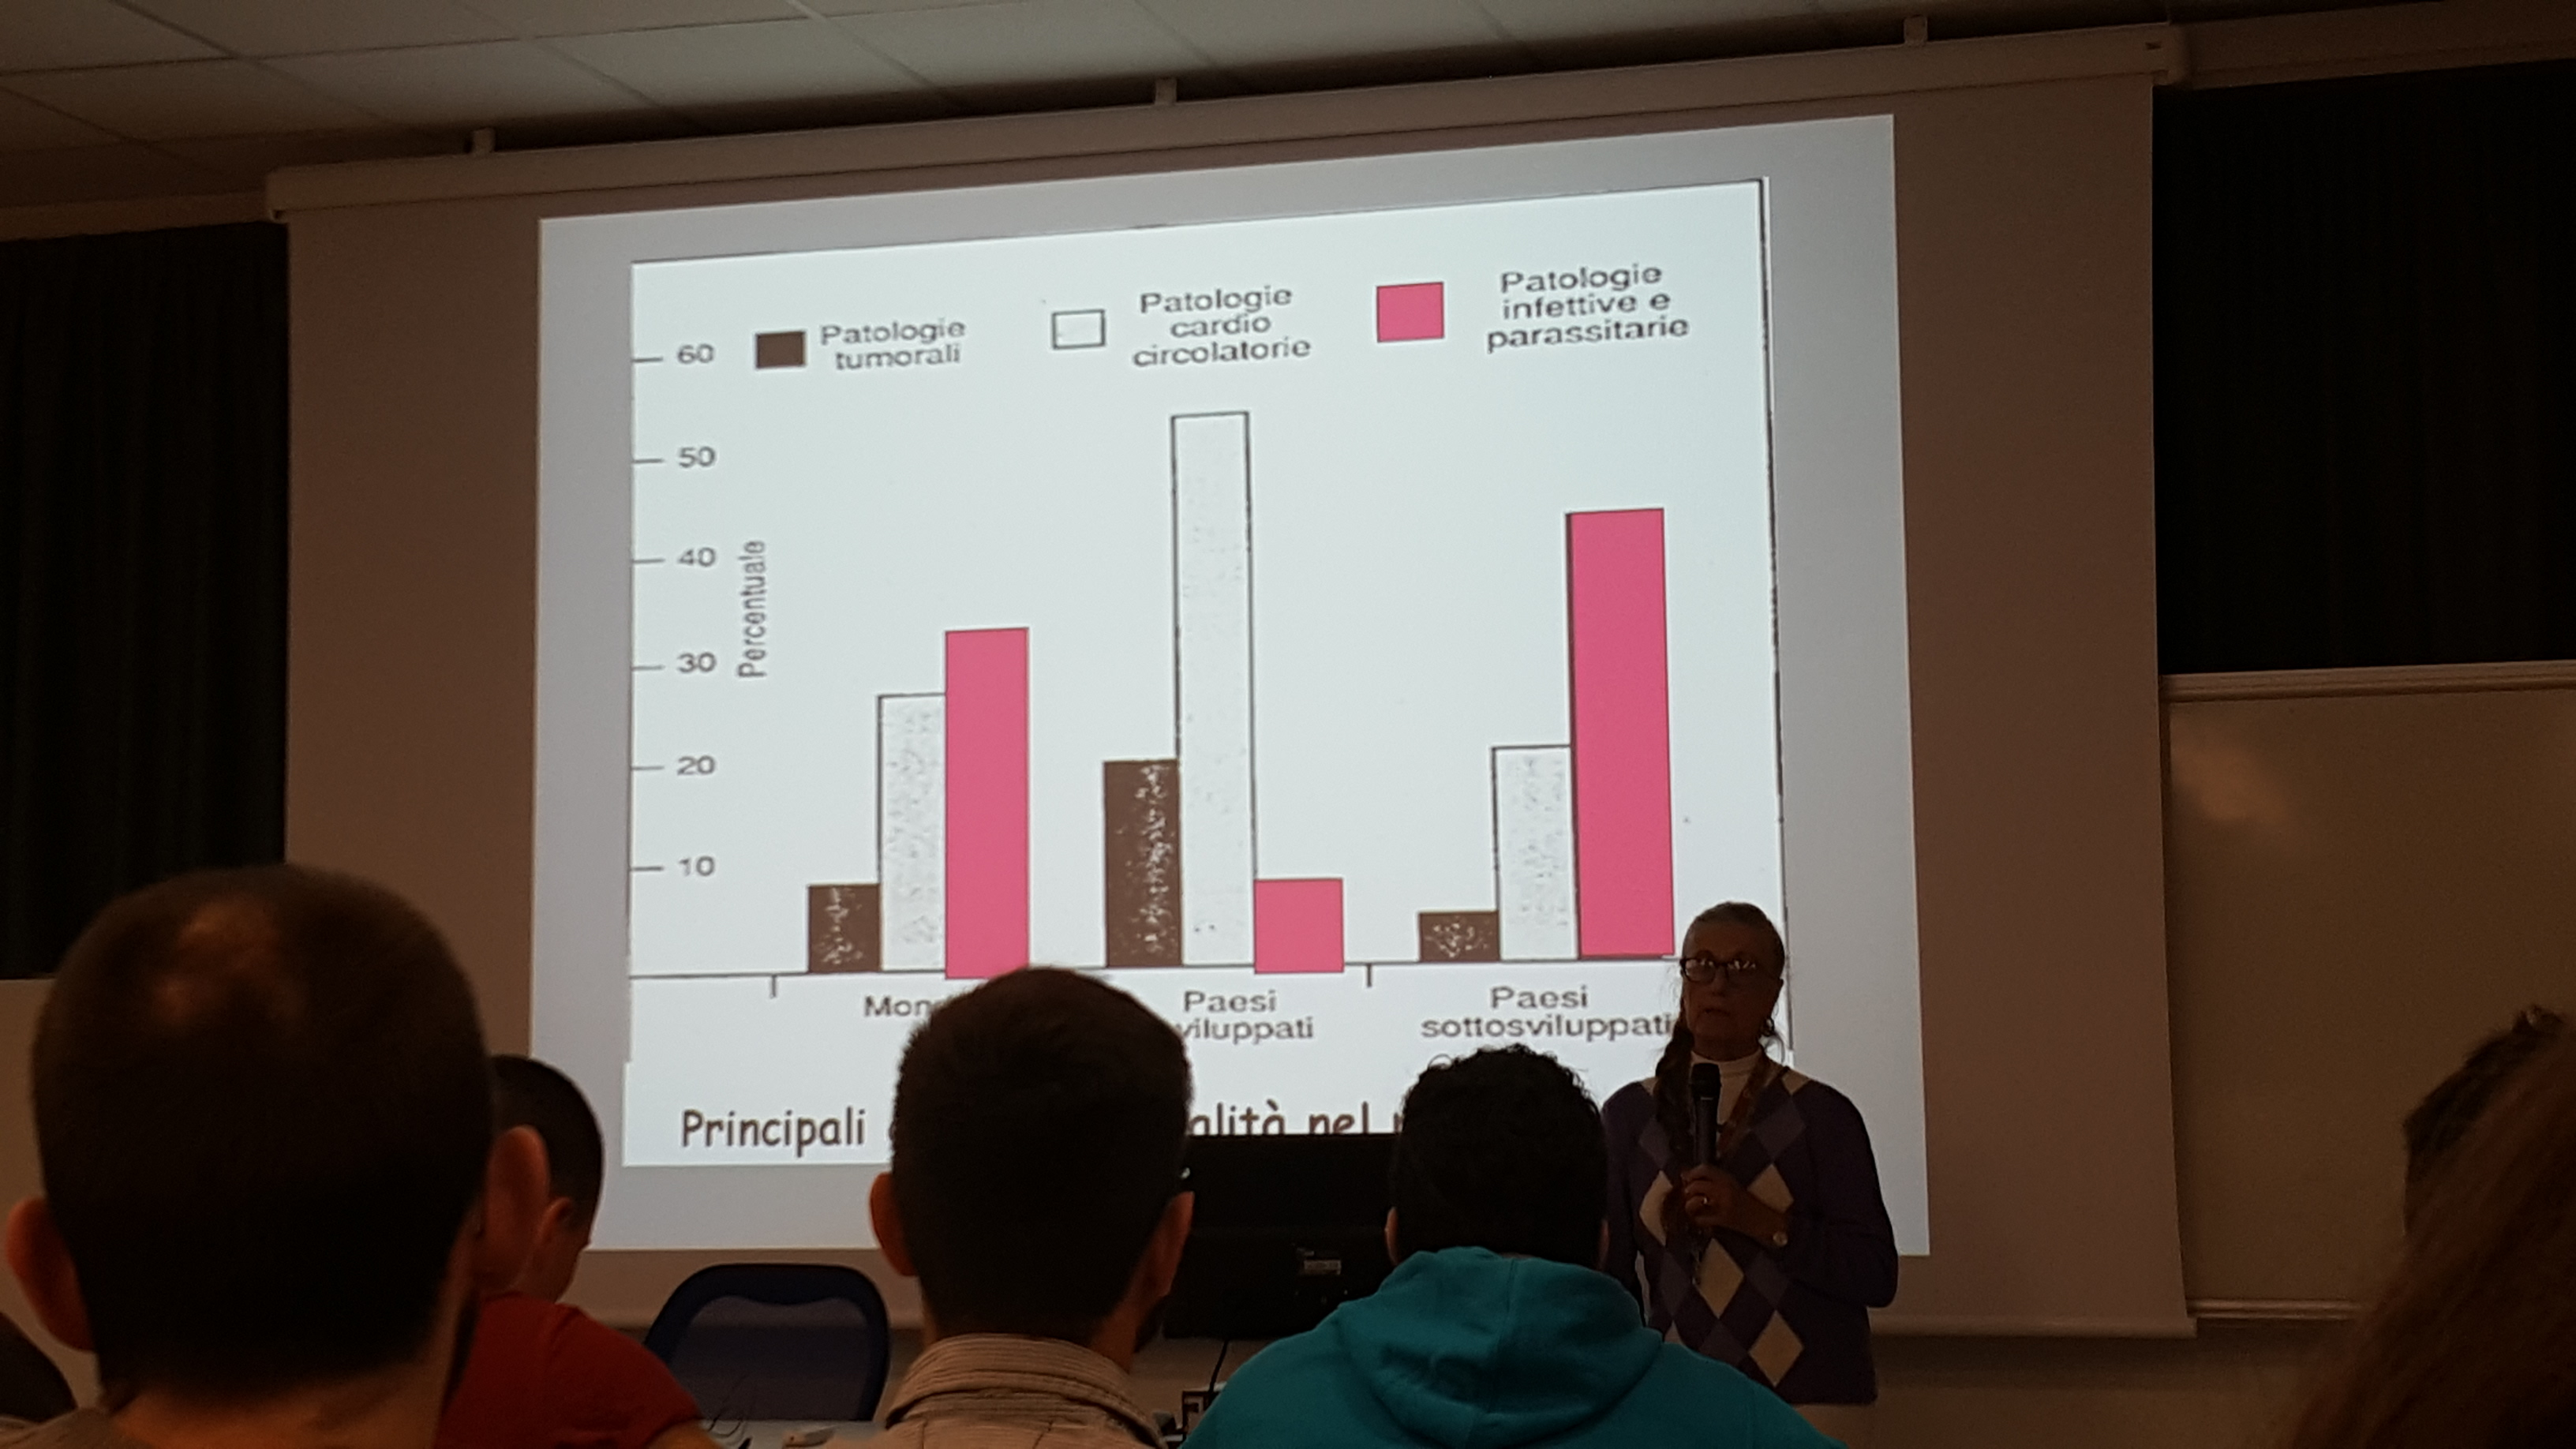
\includegraphics[width=0.8\textwidth]{06/image1.jpeg}
	\end{figure}

  Ne risulta che:
\end{itemize}

\begin{itemize}
\item
  Nei paese industrializzati le malattie infettive sono una causa
  minoritaria di morte
\item
  In alcune realtà come i paesi sottosviluppati sono ancora la prima
  causa di morte in bambini e adulti.
\end{itemize}

\begin{itemize}
\item
  Comparsa di ``nuove'' malattie e ricomparsa di malattie ritenute sotto
  controllo (TBC, ecc.). A tal proposito viene mostrato
\end{itemize}

\begin{table}
%\caption{Please write your table caption here}
\begin{tabular}{p{0.33\textwidth}p{0.33\textwidth}p{0.33\textwidth}}
\hline\noalign{\smallskip}
Anno scoperta & Agente patogeno & Malattia \\
\noalign{\smallskip}\svhline\noalign{\smallskip}
1960-1989	& Virus epatotropi (A, B, C, D, E) &	Epatiti virali \\
1973	 & Rota virus &	Gastroenteriti virali \\
1976	 & Crystosporidium parvum &	Gastroenteriti virali \\
1977	 & Ebola virus	& Febbre emorragica \\
1977 & 	Legionella pneumophila &	Legionellosi \\
1977	 & Campilobcter jejuni &	Enterite \\
1980	 & HTLV-1	& Leucemia-linfoma \\
1981 & 	Tossina Staf. Aureus	 & Sindrome shock tossico \\
1982	 & E. Coli O157:H7 & 	Colite emorragica \\
1983	 & Helicobacter pylori	& Ulcera peptidica  \\
1983 & 	Hiv	& AIDS \\
1985	 & Prioni	& vCJD \\
 & Coronavirus mutati &	SARS \\
 & Virus aviario	 & Influenza  \\
\noalign{\smallskip}\hline\noalign{\smallskip}
\end{tabular}
\end{table}

Già quanto riportato circa i nuovi patogeni spiega perché l'interesse
verso le malattie infettive è ancora attuale e l'attenzione non può
venire meno

\begin{itemize}
\item
  Comparsa/ aumento di farmaco resistenza che dà problemi sul piano
  terapeutico e preventivo perché allunga i termini di diffusione del
  patogeno. L'Italia è al primo posto per quanto riguarda la
  farmaco-resistenza di alcuni importanti patogeni
\item
  Carenza di farmaci specifici per il trattamento di molte malattie
  virali
\item
  Aumento nella popolazione di soggetti con immunodepressione legata a:

\begin{itemize}
\item
  Interventi terapeutici
\item
  Patologie tumorali
\item
  Fattori genetici
\item
  Incremento della vita media (è ``anziano'' anche il sistema
  immunitario)
\end{itemize}

\item
  Problemi economici: quanto detto fin ora ha una ricaduta considerevole
  in termini economici:

\begin{itemize}
\item
  Richieste di visite mediche
\item
  Ospedalizzazione
\item
  Richieste di farmaci
\item
  Richieste di nuovi farmaci a causa della farmaco resistenza
\item
  Cure a domicilio
\item
  Perdita di giornate di lavoro
\end{itemize}
\end{itemize}

  In termini di prevenzione delle malattie infettive abbiamo a
  disposizione tutta una serie di preparati utili e altamente specifici
  che sono i vaccini. Oggi ce ne sono molti per contrastare diverse
  patologie però ci sono malattie per le quali ad oggi ancora non
  disponiamo di vaccini efficaci e per le quali dovremmo ricorrere alle
  norme di prevenzione generale. Il piano di programmazione vaccinale è
  il documento di riferimento contenente le linee di indirizzo per la
  scelta delle strategie vaccinali e per l'inserimento di nuovi
  preparati nei gruppi di individui a maggior interesse. Si tratta di un
  piano triennale che nasce come strumento tecnico di supporto
  all'accordo stato-regione. Da ricordare infatti che dal 2001 c'è
  l'autonomia sanitaria delle regioni dallo stato però non deve esserci
  un contrasto netto con quella che è l'idea generale dello stato bensì
  la maggiore omogeneità possibile ed è ciò che questo programma vuol
  garantire.

  Viene di seguito proposto il calendario vaccinale del piano nazionale
  prevenzione vaccinale che è in forza ora.

  \begin{figure}[!ht]
\centering
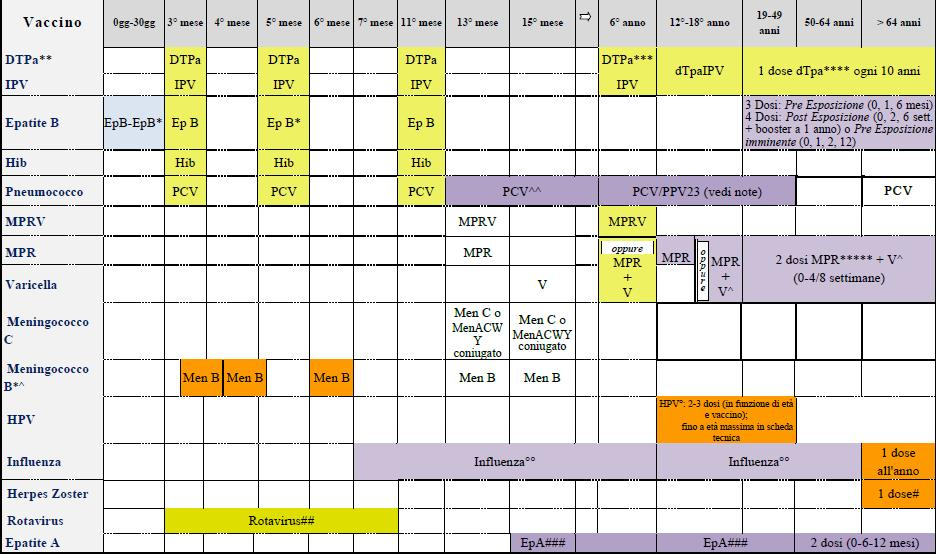
\includegraphics[width=0.7\textwidth]{06/image2.jpg}
\end{figure}

  \begin{figure}[!ht]
\centering
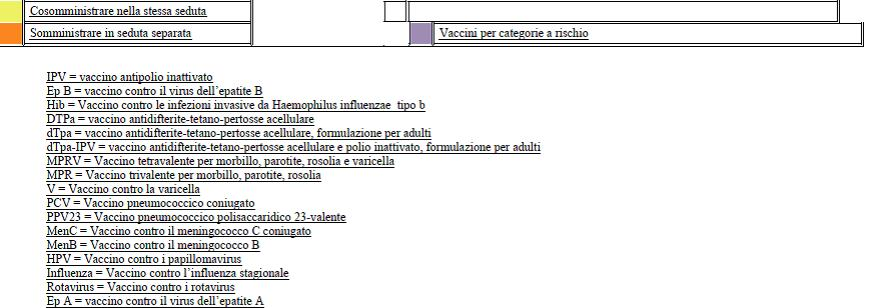
\includegraphics[width=0.7\textwidth]{06/image3.jpg}
\end{figure}

  E' interessante notare che:

\begin{itemize}
\item
  Il calendario vaccinale è inteso come calendario della vita (le
  vaccinazioni non sono limitate solo all'infanzia) perché in ogni
  momento della vita possono esserci dei momenti di fragilità, dei
  fattori di rischio, particolari situazioni in cui quel vaccino può
  trovare una sua applicazione ottimale.
\item
  La maggior parte delle applicazioni è riservata all'infanzia quando il
  bambino per la prima volta incontra i patogeni rispetto ai quali è
  quasi completamente suscettibile
\end{itemize}

  Per comodità didattica dividiamo per gruppi di popolazione i vaccini a
  disposizione. Da ricordare che è una suddivisione per nulla rigida
  tanto è vero che alcuni dei vaccini tipicamente ``dell'infanzia''
  possono trovare applicazione anche negli adulti e viceversa

\begin{itemize}

\item[1.]
  \textbf{Vaccinazioni da attuare nell'infanzia: nella prima e seconda
  infanzia}. Queste sono suddivise in obbligatorie (una legge dello
  stato prevede queste vaccinazioni a partire dal terzo mese di vita) e
  non. Queste vaccinazioni rientrano nei calendari secondo il peso loro
  attributo e sulla base della necessità di effettuarle per preservare
  il singolo e la comunità:

\begin{itemize}
\item
  Difterite
\item
  Pertosse
\item
  Tetano
\item
  Poliomielite
\item
  Epatite da HBV
\item
  Morbillo
\item
  Parotite
\item
  Rosolia
\item
  Varicella
\item
  Meningite da Haemophilus influenzae di tipo B
\item
  Meningite meningococcica
\item
  Meningite pneumococcica
\item
  Rotavirus (nuova e fortemente consigliata a livello internazionale
  nella prima infanzia)
\item
  HPV (per le ragazze in età pre-pubere)
\end{itemize}
  N.B. Quelle obbligatorie dalla riduzione perché la tendenza attuale è
  verso una maggiore liberalizzazione favorita da una migliore
  conoscenza.

\item[2.]
  \textbf{Vaccinazioni da attuare nell'età adulta o negli anziani}:

\begin{itemize}
\item
  Influenza
\item
  Infezione pneumococcica
\item
  Tubercolosi
\item
  Epatite A
\item
  Febbre tifoide
\item
  Colera
\item
  Rabbia
\item
  Tetano
\item
  Meningite meningococcica (l'infezione meningococcica ha un classico
  andamento bimodale quindi un primo picco nell'infezione e uno
  successivo in età più avanzata)
\item
  Epatite B (in caso non sia stata effettuata nella prima infanzia)
\end{itemize}
  Alcune di queste (Epatite A, Febbre tifoide, Colera e Rabbia) sono
  consigliate a seconda delle condizioni di vita
\end{itemize}
  Infine ricordiamo che ci sono vaccini anche per le patologie tumorali:

\begin{itemize}
\item
  Vaccino per l'epatite B: prevenendo l'infezione virale, preveniamo una
  delle più severe conseguenze dell'infezione che è il carcinoma epatico
\item
  Vaccino per HPV
\end{itemize}

\subsection{Difterite}

  Si tratta di una malattia infettiva e contagiosa di cui l'agente
  eziologico è il batterio Corynebacterium Diphteriae. Il contagio
  avviene per lo più per via aerea per aerosol o con oggetti contaminati
  quindi il malato di difterite è altamente contagioso e la trasmissione
  avviene per contagio interumano.

\subsubsection{Epidemiologia}

  Gli ultimi casi in Italia risalgono al periodo 1991-1996 e si è
  trattato di 4 casi di bambini non vaccinati mentre nella regione OMS
  Europa nel 1995 c'è stato un focolaio epidemico importante che ha reso
  questa regione responsabile de 90\% dei casi di difterite registrati
  in quell'anno. Questi casi in Europa furono concentrati nel territori
  della vecchia URSS in fase di rinnovamento economico e sanitario: la
  situazione sul piano sanitario era ottima, ma si è venuta a
  determinare una disorganizzazione dei servizi sanitari a seguito dei
  cambiamenti politici con interruzione della pratica vaccinale da cui
  questi focolai epidemici. La prevalenza nella popolazione mondiale è
  diversa se consideriamo paesi industrializzati e paesi in via di
  sviluppo. Nei paesi industrializzati è stata debellata pressoché, ma
  non eradicata: il patogeno è ancora presente nella popolazione quindi
  non c'è la malattia, ma la possibilità che la malattia si ripresenti.

  L'epidemiologia risultante deriva dal bilancio tra portatori sani e
  soggetti suscettibili che possono favorire la propagazione del
  patogeno. I portatori sani sono stati fortemente ridotti
  dall'intervento preventivo vaccinale ampiamente diffuso e attivo dagli
  anni 30. Tuttavia questi portatori sani se pur ridotti, sono ancora
  presenti nella popolazione. I soggetti suscettibili sono invece
  aumentati nei paesi industrializzati a causa della riduzione
  dell'immunità anticorpale perché l'immunità si concretizzi
  nell'infanzia grazie al vaccino e poi tende a perdersi se non ci sono
  nuovi stimoli artificiali ovvero vaccini o naturali ovvero il patogeno
  che non c'è perché circola poco come patogeno. Questi ospiti
  suscettibili sono diffusi per lo più tra gli adulti e gli anziani
  ovviamente.

\begin{itemize}
\item
  L'altro aspetto da considerare è quello legato alle massicce
  emigrazioni di soggetti che provengono da aree endemiche e sono
  portatori sani e quini possono potenzialmente reintrodurre il
  patogeno.
\item
  Infine in molti dei paesi in via di sviluppo dove l'infezione non è
  pressoché debellata, ci sono delle condizioni politiche fragili per
  cui la pratica vaccinale (se pur abbastanza diffusa sul pianeta) si
  riduce o diviene saltuaria creando una condizione di non immunità.
\end{itemize}

  Quanto detto rende ragione del fatto che nella nostra realtà la
  difterite è un evento sporadico, eccezionale e quando si presenta lo
  fa sotto forma di piccoli focolai in piccole comunità chiuse in cui
  sono presenti ospiti suscettibili. Più grave è la ricomparsa di
  focolai epidemici come accadde nel 1995. Nonostante la bassa morbosità
  è una malattia gravata ancora da elevata mortalità.

  Nei paese in via di sviluppo invece è una malattia dell'infanzia, ad
  andamento endemico e gravata da elevata mortalità e ancora da elevata
  morbosità. Queste realtà sono quelle da cui il patogeno può diffondere
  ad altre realtà attraverso la figura del portatore sano (ad esempio a
  seguito di viaggi oltre che flussi migratori).
  
\subsubsection{Modalità di trasmissione}

  Il caso della difterite è emblematico del problema delle malattie
  infettive oggi: molte sono le malattie poste sotto controllo da
  decenni però se esiste ancora il patogeno in qualche punto del
  pianete, in qualche popolazione allora c'è la possibilità che la
  malattia si ripresenti. E' importante ricordare che questo è possibile
  se nella popolazione rimangono soggetti suscettibili all'infezione: se
  c'è la possibilità che il patogeno rientri e questi trova un soggetto
  (ospite) non immune, questo fa da volano per l'ingresso del patogeno
  nella comunità dove potrà trovare altri ospiti suscettibili. La
  certezza di non avere più determinate malattie infettive deriva solo
  dall'eradicazione che ad oggi è stata ottenuta solo per il vaiolo
  mentre si è probabilmente molto vicini a raggiungerla per la
  poliomielite invece è in atto per morbillo, rosolia e parotide.

\subsubsection{Modalità di trasmissione e contagio}

  Il contagio avviene per via aerea per aerosol o con oggetti
  contaminati. Il batterio non è invasivo, si localizza nella sede
  d'ingresso e moltiplica negli epiteli dove si è localizzato. L'azione
  patogena è legata prevalentemente all'esotossina infatti la difterite
  è considerata una tossiemia. La tossina difterica è una delle tre
  grandi esotossine che temiamo insieme alla tetanica e botulinica.

  La tossina è dimerica (A+B) e ha un'azione necrotizzante a livello
  locale mentre diffonde per via ematica agendo a distanza su organi e
  tessuti da cui tutta la sintomatologia indotta dalla difterite. La
  tossina penetra all'interno della cellula dopo interazione della
  subunità B con un recettore specifico e successiva endocitosi mediata
  dal recettore. Il legame della subunità B al recettore è
  irreversibile. Il ph acido delle vescicole di endocitosi rompe i ponti
  disolfuro A+B. A questo punto il monomero A può uscire e raggiunger il
  citoplasma e interagire con il fattore di allungamento EF2
  interrompendo la sintesi proteica e causando la morte della cellula in
  poche ore. Questa è una caratteristica non di tutti i ceppi, ma solo
  di quelli che hanno integrato nel proprio genoma il fago \emph{beta}
  come profago col gene \emph{tox+.}

  Per quanto riguarda la potenza: 25 ng sottocute in una cavia di 250 gr
  provocano la morte in 4-5gg e questa è dunque la dose minima letale.

  \begin{figure}[!ht]
\centering
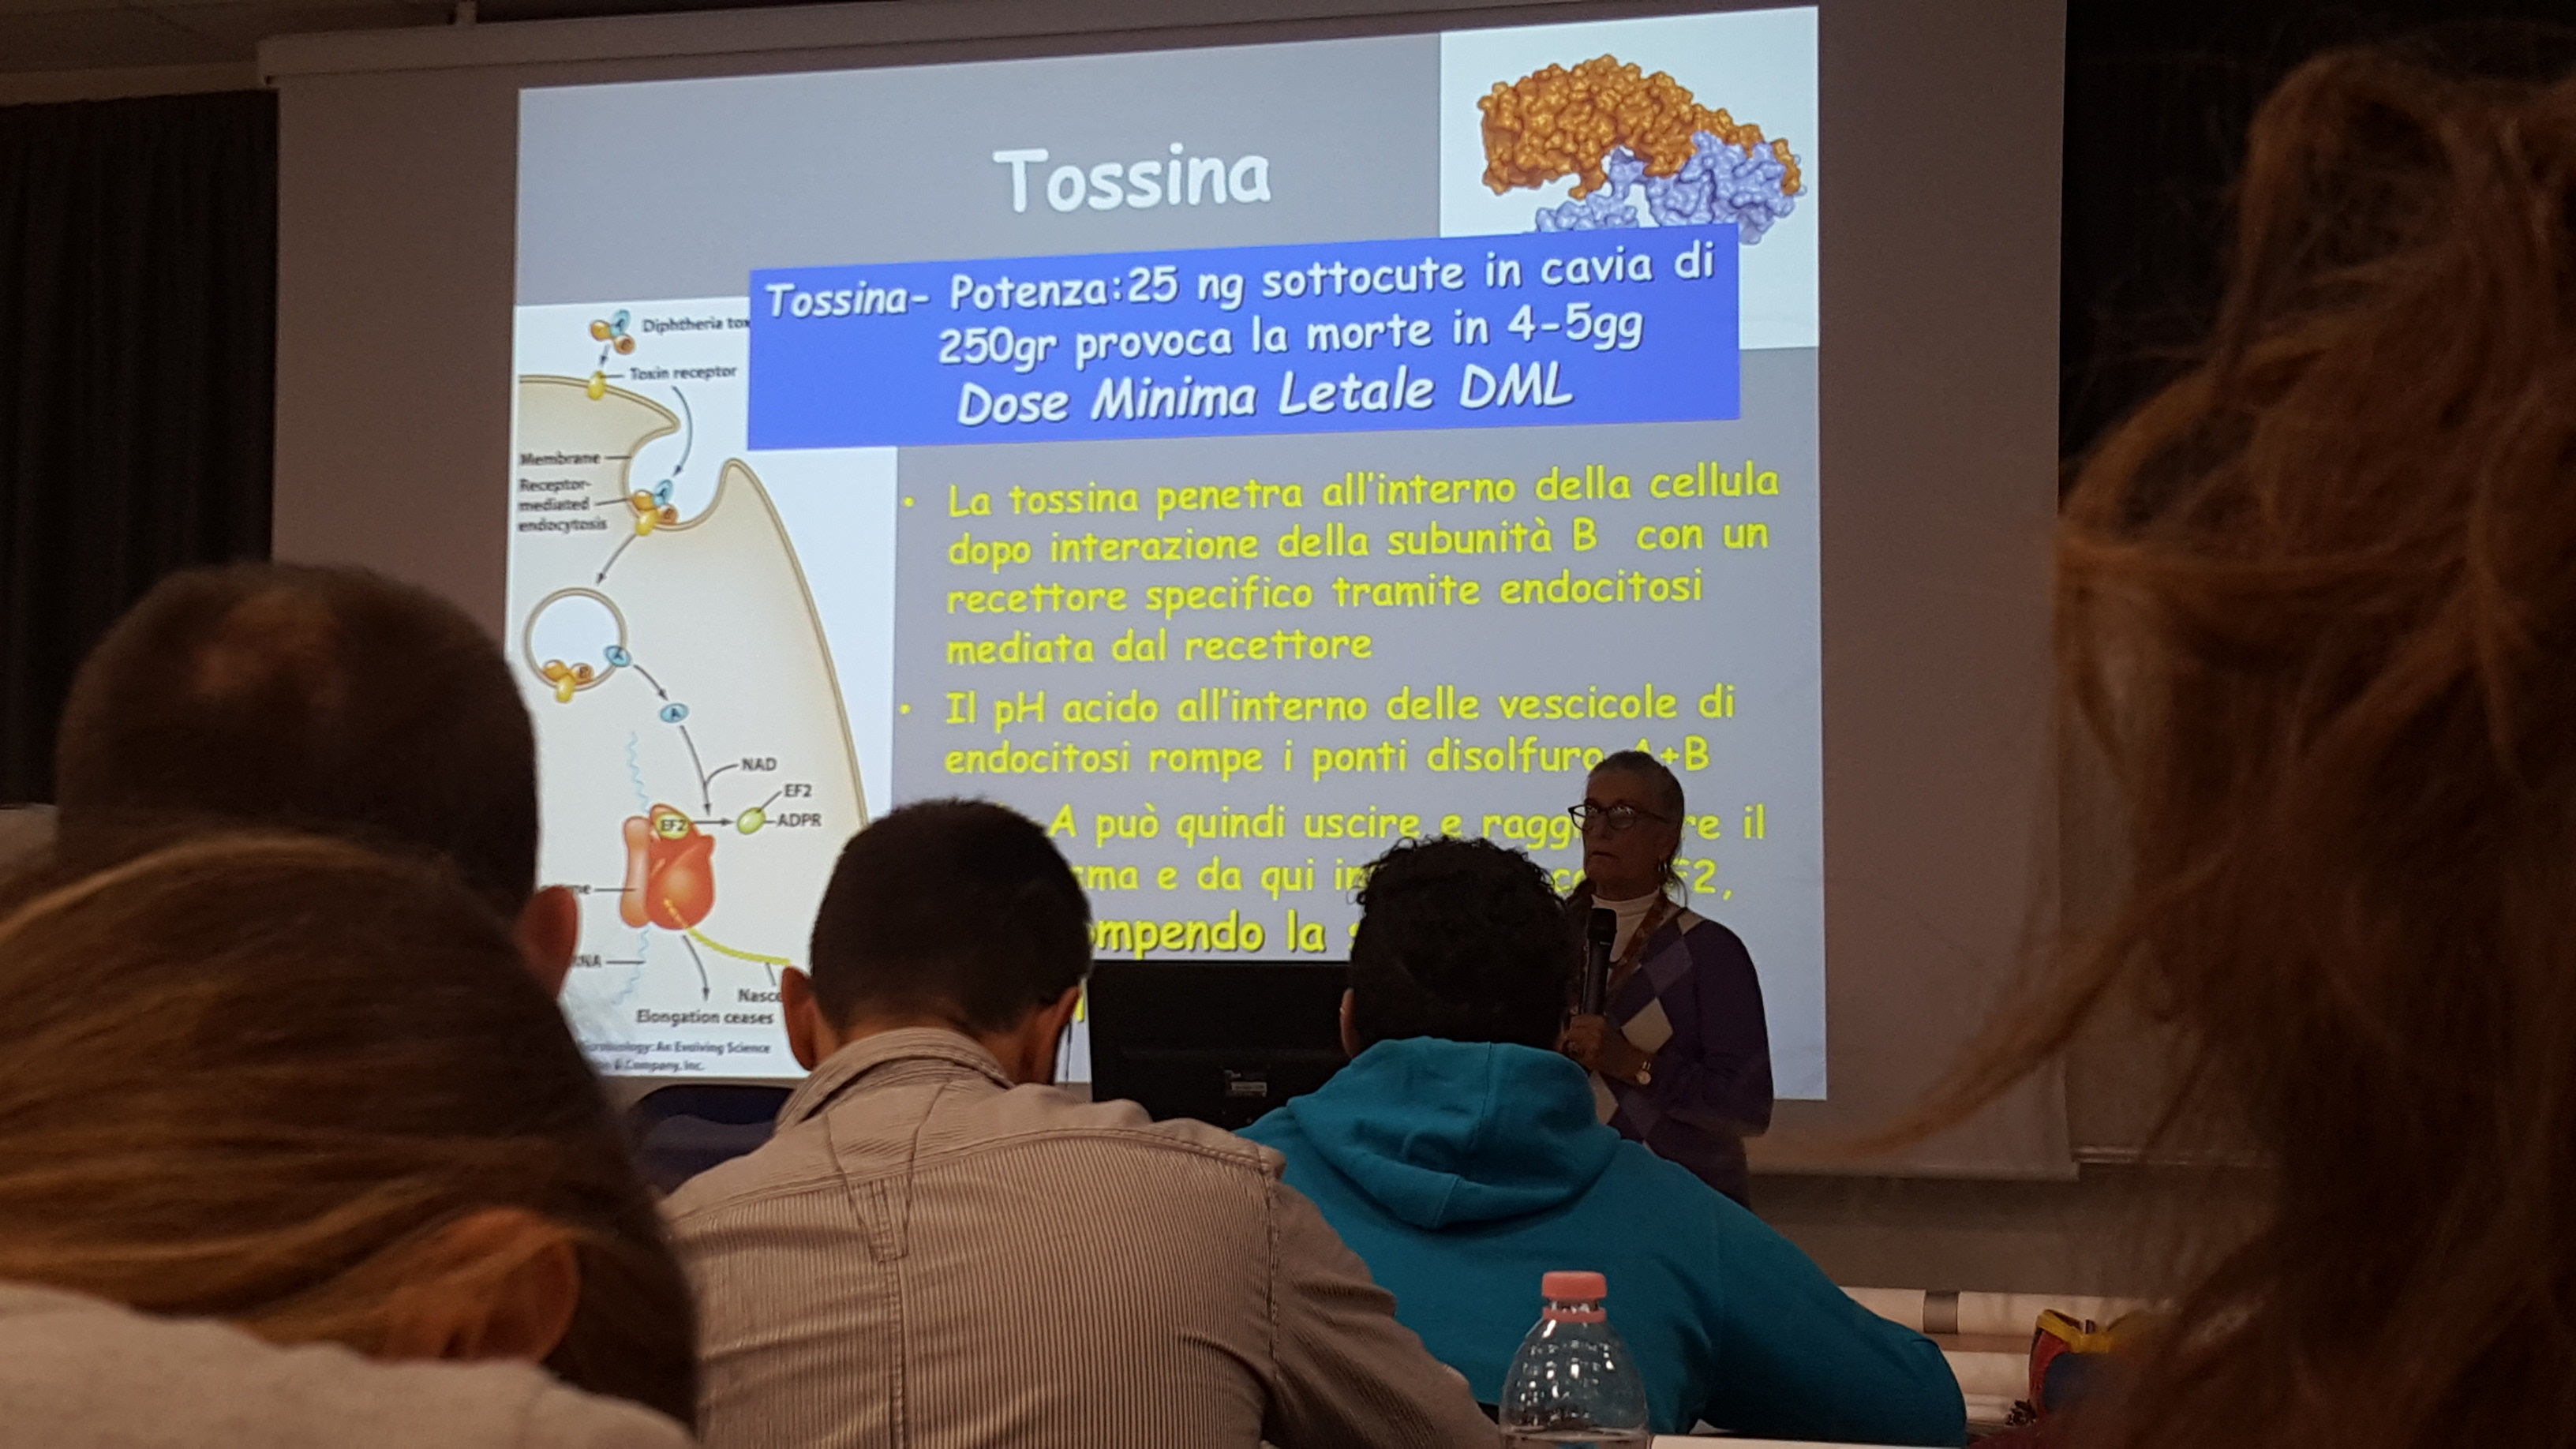
\includegraphics[width=0.7\textwidth]{06/image4.jpeg}
\end{figure}

\subsubsection{Clinica}
  La malattia ha un periodo di incubazione di circa 8 giorni e le sedi
  classicamente coinvolte sono quelle dell'apparato respiratorio:

\begin{itemize}
\item
  Faringe
\item
  Laringe
\item
  Naso
\end{itemize}
  C'è la possibilità di un coinvolgimento anche di altre sedi però il
  coinvolgimento classico e più impegnativo è proprio quello delle vie
  aeree.

  La forma più comune è quella faringea perché la ricca
  vascolarizzazione facilita la diffusione della tossina. Dopo il
  periodo di incubazione si ha la caratteristica comparsa di
  pseudo-membrane bianco-grigiastre fortemente aderenti ai tessuti
  sottostanti, edema che dà anche un coinvolgimento di tipo meccanico
  nell'atto respiratorio e adenopatia.

  La forma laringea spesso segue la faringea però più raramente è
  indipendente. In questo caso la dinamica meccanica è molto impegnativa
  perché portando all'ostruzione del lume, avremo difficoltà
  respiratoria fino all'insufficienza respiratoria vera e propria.

  La rinite non ha un gran peso tanto è vero che a volte passa
  addirittura inosservata però è importante perché anche in questa fase
  il soggetto è contagioso ed è quindi problematica proprio in relazione
  all'elevata contagiosità. In passato era tipica dei bambini.

  A sintomi locali (edema, restringimento del lume, ecc.) si affianca la
  componente più grave della malattia che è la tossiemia generalizzata
  che causa:

\begin{itemize}
\item
  Alterazione cardiocircolatorie che portano a sofferenza cardiaca. La
  miocardite si presenta in una quota non trascurabile di casi (circa 1/4)
  e porta inevitabilmente a morte. La miocardite determina danno
  miocellulare diretto e si verifica nel 10-25\% dei casi. Si manifesta
  entro 3-7 giorni dall'esordio dei sintomi. Quando si verifica è
  solitamente ed inevitabilmente fatale
\item
  Alterazioni renali che evolvono vero la necrosi tubulare
\item
  Paralisi a carico delle sedi muscolari coinvolte quindi muscoli
  faringei, laringei e oculari. Le complicanze respiratorie hanno una
  letalità nel 5-10\% dei casi
\item
  Coinvolgimento del sistema nervoso centrale. La letalità è legata alla
  tossicità neurologica nel 20\% dei casi
\end{itemize}

\subsubsection{Prevenzione e profilassi}

  L' accertamento diagnostico è importante per riconoscere i soggetti
  infettanti infatti nella difterite abbiamo due figure: malato e
  portatore sano (precoce, convalescente e cronico quindi anche a
  guarigione avvenuta). In passato si stimava che per ogni malato ci
  fossero 20 portatori sani e questo giustifica l'elevata diffusione e
  contagiosità della malattia. La legge prevede sul piano della
  prevenzione:

\begin{itemize}
\item
  Notifica obbligatoria di classe 1: nella nostra realtà sanitaria un
  caso di difterite è un caso sentinella
\item
  Isolamento del malato fino a 3 giorni per la gravità e il rischio di
  contagio
\item
  Tamponi faringei: controllo post-malattia del malato per verificare
  che non sia un eliminatore o portatore cronico mediante l'esame di 3
  tamponi faringei a distanza di 2 giorni che devono risultare negativi.
  Questo consente il re-inserimento in società (pensate in passato
  quando ancora esistevano focolai epidemici e i bambini soprattutto
  dovevano essere reinseriti in società e contesti molto affollati tipo
  scuole, colonie ecc.)
\item
  Controllo dei contatti per verificare eventuali contagi e altri casi
  di malattia
\item
  Inchiesta epidemiologica che è parte integrante del programma di
  sorveglianza sanitaria e si pone l'obiettivo di individuare i
  portatori sani e suscettibili attorno al malato. Tale indagine si
  avvale di opportuni accertamenti e indagini diagnostiche
\end{itemize}
  E' discretamente resistente come batterio e quindi richiede molta
  attenzione nella disinfezione di ambiente, suppellettili e mani,
  disinfezione continua a letto del malato. Disponiamo di un efficace
  vaccino che è l'anatossina ovvero la tossina privata del potere
  tossico (vecchia tecnica di Ramon degli anni 20 che è stata
  ammodernata solo dal punto di vista metodologico).

  Un vaccino singolo non esiste anzi non è mai esistito perché fin da
  subito è stato associato alla vaccinazione anti-tetanica dal momento
  che la tossina è abbastanza simili e i preparati facili da maneggiare
  insieme. Ad oggi disponiamo di:

\begin{itemize}
\item
  Vaccino a dose completa (indicato con la lettera maiuscola)
\item
  Vaccino a dose ridotta per l'adulto perché più reattogena e può dare
  problemi di sensibilità.
\end{itemize}
  La vaccinazione è obbligatoria dagli anni 30 e abbiamo a disposizione
  vaccini penta e esavalenti tutti contenenti sia l'anatossina difterica
  che tetanica.

  Più recente è invece il trivalente (tetano, difterite, pertosse) che è
  indicato per giovani adulti e adulti e che prevede una dose ridotta di
  difterite. La motivazione che ha portato all'introduzione di questo
  nuovo vaccino è proprio il fatto che nella popolazione adulta c'è una
  quota rilevante di siero positivo o comunque di suscettibili per
  riduzione dell'immunità acquisita durante l'infanzia. Si sfrutta in
  questo caso l'effetto trainante del tetano e si aggiunge anche il
  vaccino per la difterite e la pertosse. C'è a disposizione un
  preparato contente oltre i tre anche il vaccino per la poliomielite
  però questo è destinato a soggetti potenzialmente a rischio per questa
  infezione.

  Scheda vaccinale: terzo, quinto e undicesimo mese (tre dosi nel primo
  anno di vita) e un primo richiamo che completa il ciclo all'ingresso
  nella scuola (intorno ai 6 anni) e a cui si è aggiunto negli ultimi
  anni un ulteriore richiamo più o meno alla fine dell'obbligo
  scolastico circa intorno ai 12 anni.

  Il trivalente invece serve per rinnovare l'immunità negli adulti. La
  strategia attuale in Italia è quella di vaccinare gli adulti per
  mantenere il titolo anticorpale il più alto possibile sfruttando tutte
  le occasioni in cui c'è vaccinazione per il tetano che è più diffusa
  anche in relazione a particolari figure professionali. Viene a tal
  proposito presentato lo studio ESEN che si poneva come obiettivo
  quello di valutare la prevalenza di sieronegativi nella popolazione di
  adulti di età superiore ai 30 anni.

  \begin{figure}[!ht]
\centering
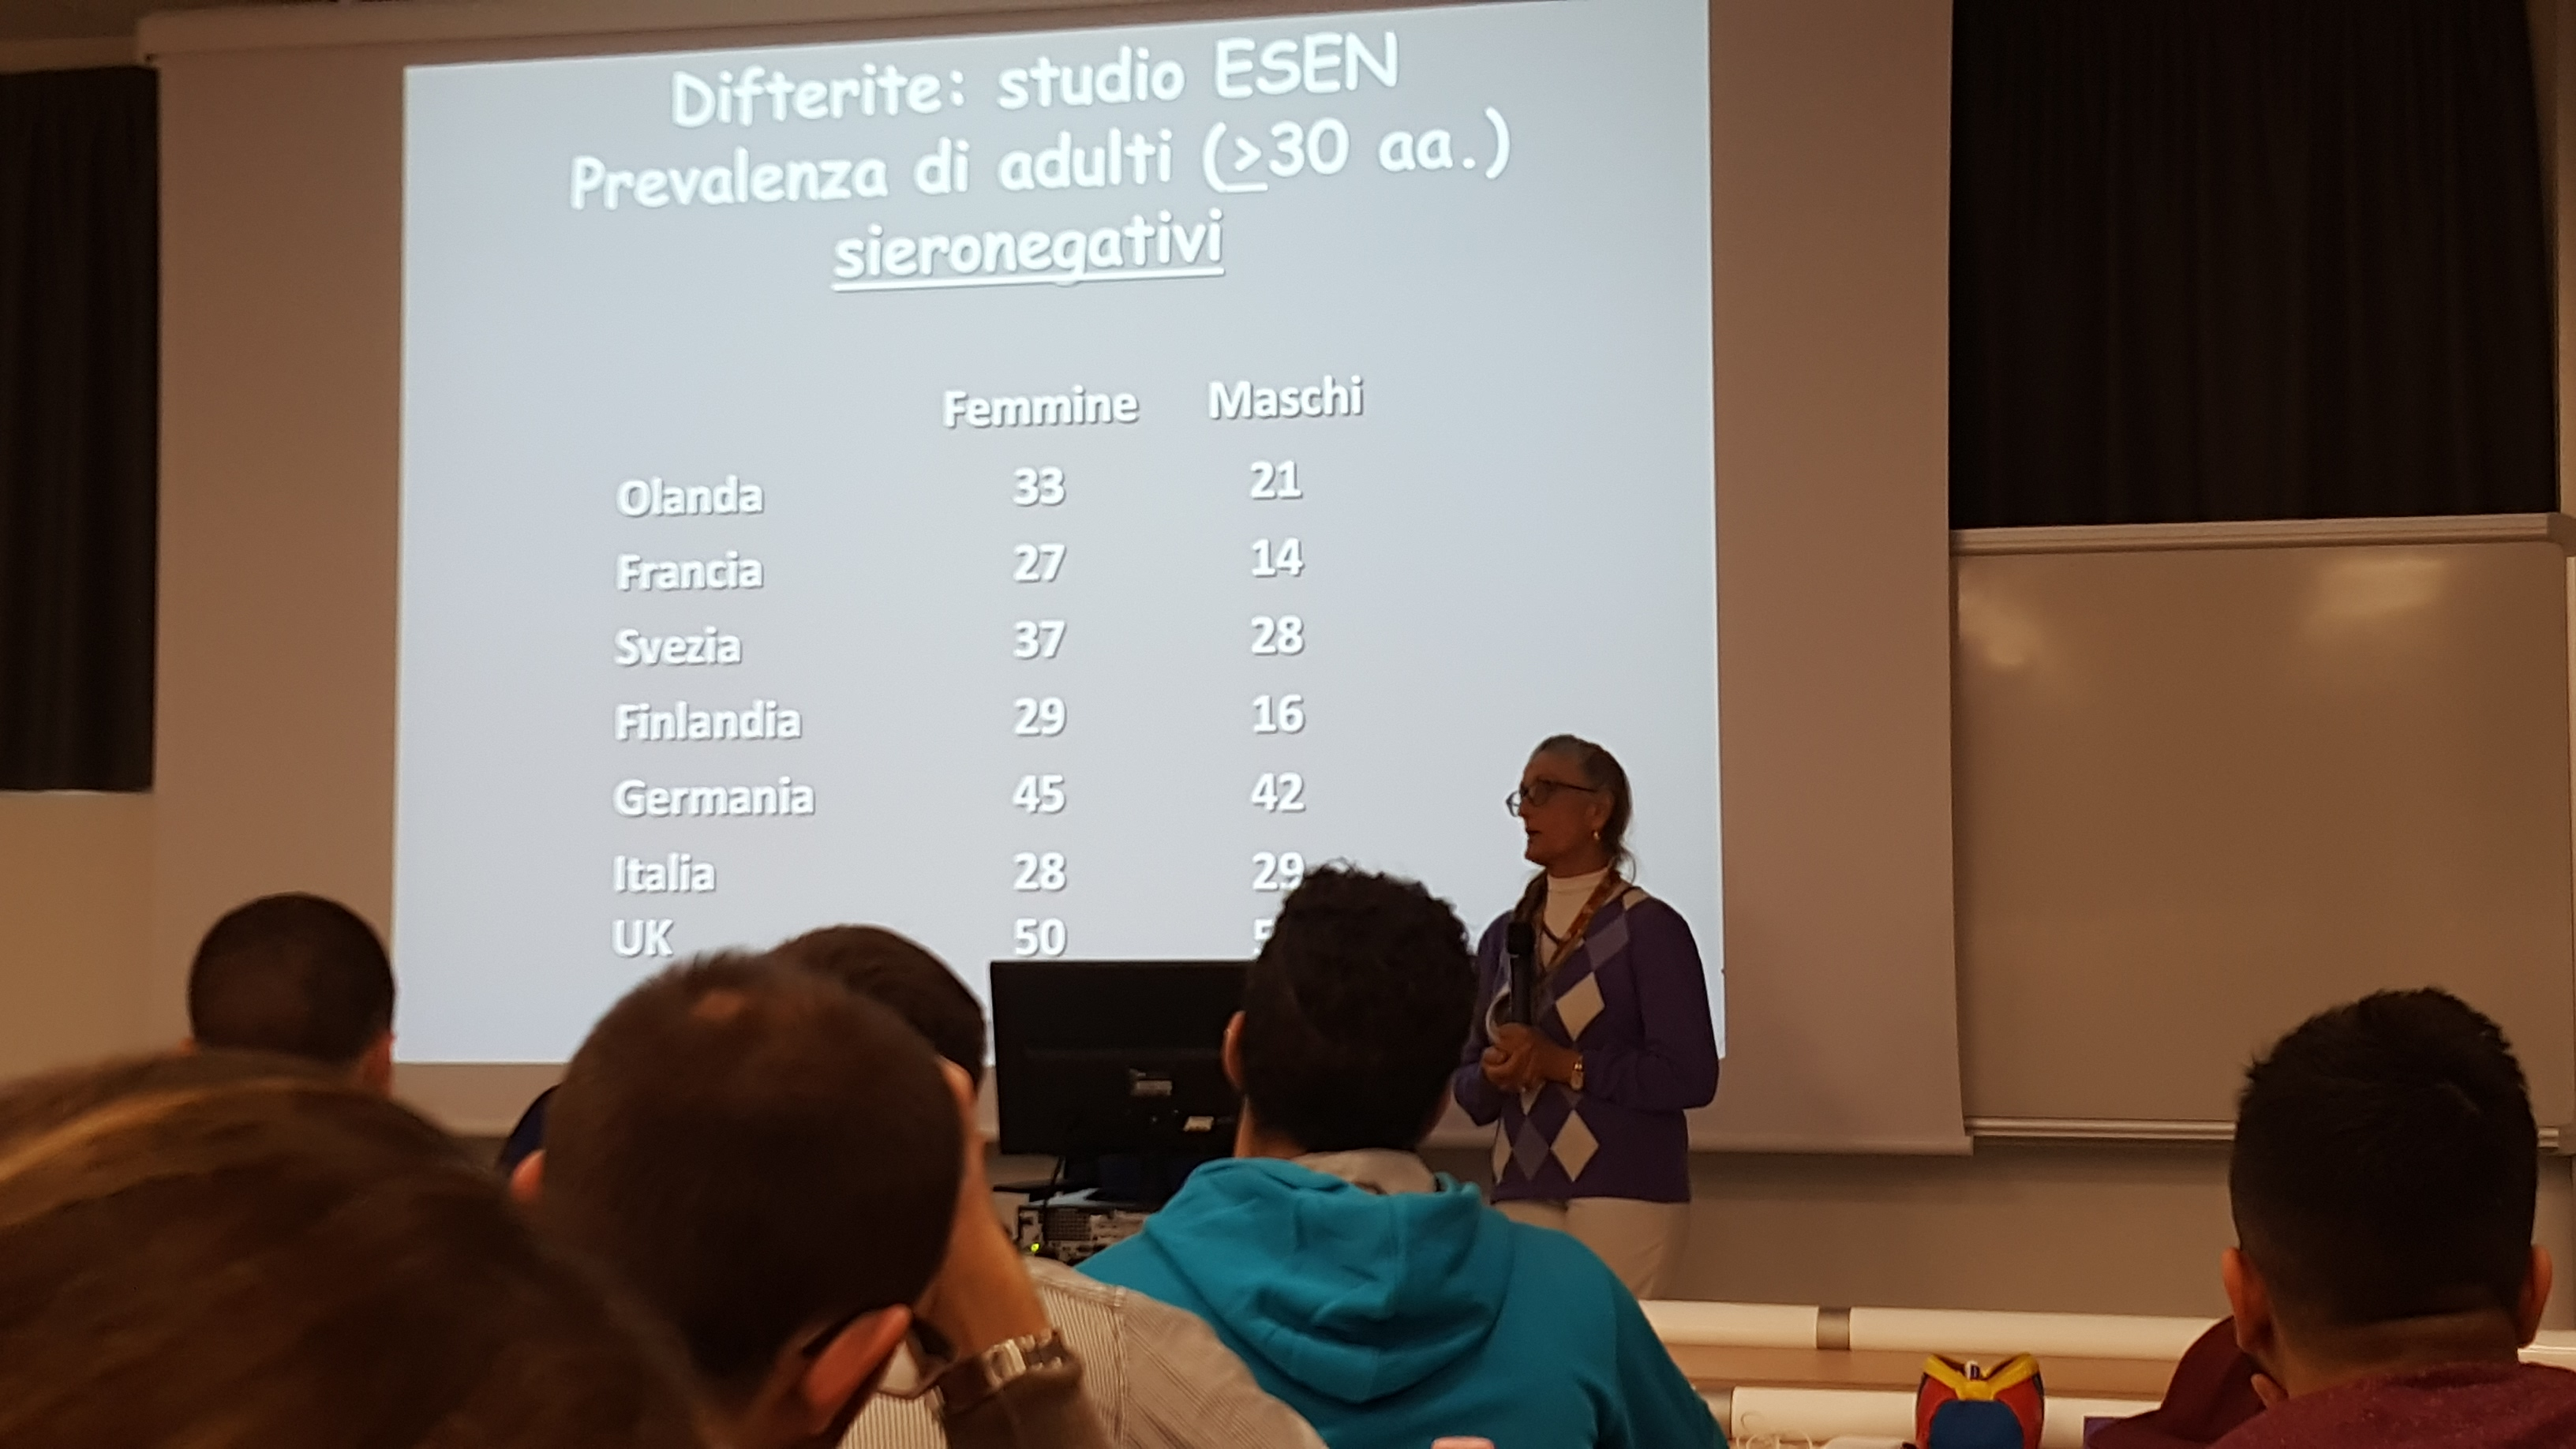
\includegraphics[width=0.7\textwidth]{06/image5.jpeg}
\end{figure}

  La percentuale di sieronegativi nella popolazione al di sopra dei 30
  anni è del 50\% in certe realtà sanitarie mentre è intorno al 30\% da
  noi quindi poco meglio e giustifica questa nuova strategia

  Una vaccinazione estesa al di sopra del 90\% della popolazione ci
  garantisce che il patogeno non arrivi agli ospiti suscettibili:
  secondo l'OMS il rischio di difterite viene abbattuto se abbiamo una
  immunizzazione della popolazione infantile oltre il 90\% (95\%) e
  negli adulti oltre il 75\%. L'Obiettivo internazionale è
  l'eradicazione nei paesi industrializzata e la sporadicità in quelli
  in via di sviluppo.

  Si tratta di una vaccinazione di efficacia molto elevata. Gli effetti
  collaterali sono di tipo locale e sono inevitabili dal momento che è
  un vaccino adiuvato quindi il potenziatore dell'immunità, che in
  questo caso è l'idrossido di alluminio, crea un deposito in sede di
  somministrazione che da infiammazione assolutamente trascurabile e
  solo raramente abbiamo della reazioni generali (febbre sopra i 38). Va
  considerata la possibilità di reazioni di tipo allergico se viene data
  la dose totale sopra i 6 anni. Chi non va vaccinato? Quasi nessuno in
  realtà ad eccezione di:

\begin{itemize}
\item
  Chi ha delle reazioni allergiche alla prima dose e quindi non riceverà
  la seconda
\item
  Le persona malata perché si vaccinano solo i sani
\end{itemize}

  La vaccinazione è una tecnica di prevenzione nel tempo, rivolta al
  futuro qualora il soggetto incontrasse il patogeno mentre
  l'immunoprofilassi è proiettata nell'immediato nel caso in cui vi sia
  una condizione di rischio chiaro o comunque quasi certo. Inizialmente
  studiate per la terapia e oggi utilizzate nella prevenzione, le IgG
  sono i preparati utilizzati nell'immunoprofilassi. Oggi si utilizzano
  IgG umane e non più di origine animale. Ricordando che l'aggancio alla
  cellula è irreversibile, la somministrazione delle immunoglobuline
  deve essere tempestiva così che queste possano agire prima del legame
  della tossina al recettore. L'effetto delle immunoglobuline è a breve
  termine perché nell'arco di 3-4 settimane la concentrazione ematica
  rientra perché eliminate in quanto qualcosa di estraneo

\subsection{Tetano}

  Malattia infettiva acuta non contagiosa (a differenza della difterite
  che è a contagio interumano) di cui è agente eziologico Clostridium
  tetani. Il malato di tetano non è contagioso e la diffusione della
  malattia è legata alla persistenza del patogeno nell'ambiente sotto
  forma di spora ed è quindi dall'ambiente che noi acquisiamo
  l'infezione. Per quanto riguarda le modalità di trasmissione è
  necessaria una precisazione perché siamo di fronte a un tipo di
  infezione in cui serbatoio e sorgente non coincidono:

\begin{itemize}
\item
  Il serbatoio è l'habitat di sopravvivenza del patogeno
\item
  La sorgente è l'habitat di sopravvivenza del patogeno da cui può anche
  uscire autonomamente
\end{itemize}
  Il serbatoio sono tutti gli erbivori che albergano Clostridium tetani
  nell'intestino. Il batterio viene eliminato nell'ambiente sotto forma
  di spora e noi ci infettiamo perché penetra materiale ambientale in
  ferite, lesione quindi la sorgente è l'ambiente. L'uomo è
  semplicemente un ospite occasionale, un incontro fortuito legato per
  lo più a traumi (almeno in Italia) però ci sono dei fattori che
  favoriscono l'infezione:

\begin{itemize}
\item
  Il tipo di lesione: più è profonda, più è contaminata
\item
  L'eventuale sovra-infezione da parte di altri patogeni
\end{itemize}
  Tali condizioni possono determinare o meno condizioni favorevoli alla
  germinazione. Se non ci sono le condizioni di germinazione, non ho il
  tetano. Più pericolose sono le ferite penetranti, profonde e non
  sanguinanti perché se c'è sangue, c'è pulizia della ferita.

  E' una malattia estremamente rara, ma altrettanto grave e per la quale
  non esiste un'immunità naturale: sono pochissimi i malati che
  sopravvivono all'infezione e se lo fanno, non producono anticorpi
  protettivi utili a proteggersi nel tempo e paradossalmente potrebbero
  infettarsi nuovamente. La sola protezione efficace è quella conferita
  dall'immunità artificiale ovvero dalla vaccinazione. E' un vaccino
  utile per tutta la vita perché il rischio di contrarre il clostridio
  permane per tutta la vita infatti sono previsti degli step organizzati
  di vaccinazione e richiamo della vaccinazione.

\subsubsection{Epidemiologia}

  E' un'infezione diffusa in tutto il mondo, non c'è un'età prevalente
  mentre c'è un sesso prevalente che è quello femminile. E' presene in
  tutto il mondo però:

\begin{itemize}
\item
  Nei paese industrializzati abbiamo prevalentemente la forma adulta che
  è quella traumatica
\item
  Nei paese in via di sviluppo abbiamo anche il tetano puerperale e
  neonatale e abbiamo la massima letalità
\end{itemize}
  Parliamo di distribuzione temporale perché pur non essendoci
  propriamente una stagionalità, è un'infezione che acquisiamo
  dall'ambiente quindi più tempo trascorriamo all'aperto e maggiore è la
  probabilità di contrarla perciò i periodi in cui trascorriamo più
  tempo all'aperto, sono anche quelli in cui siamo più a rischio.
  Inoltre ci sono categorie professionali che sono più a rischio:
  metalmeccanici, muratori o che hanno rapporti con il terreno.
  Ricordando che il serbatoio del batterio sono tutti gli erbivori,
  possiamo facilmente capire perché prima questa infezione fosse
  dilagante: questi animali erano molto più diffusi e la conseguente
  fecalizzazione dell'ambiente esponeva a rischio soprattutto gli uomini
  a causa delle loro attività professionali. E' cambiata in maniera
  netta l'incidenza con le vaccinazioni: c'è stata una progressiva
  riduzione e un'inversione di tendenza perché oggi nei paese
  industrializzati sono più colpite le donne rispetto a gli uomini

  \begin{figure}[!ht]
\centering
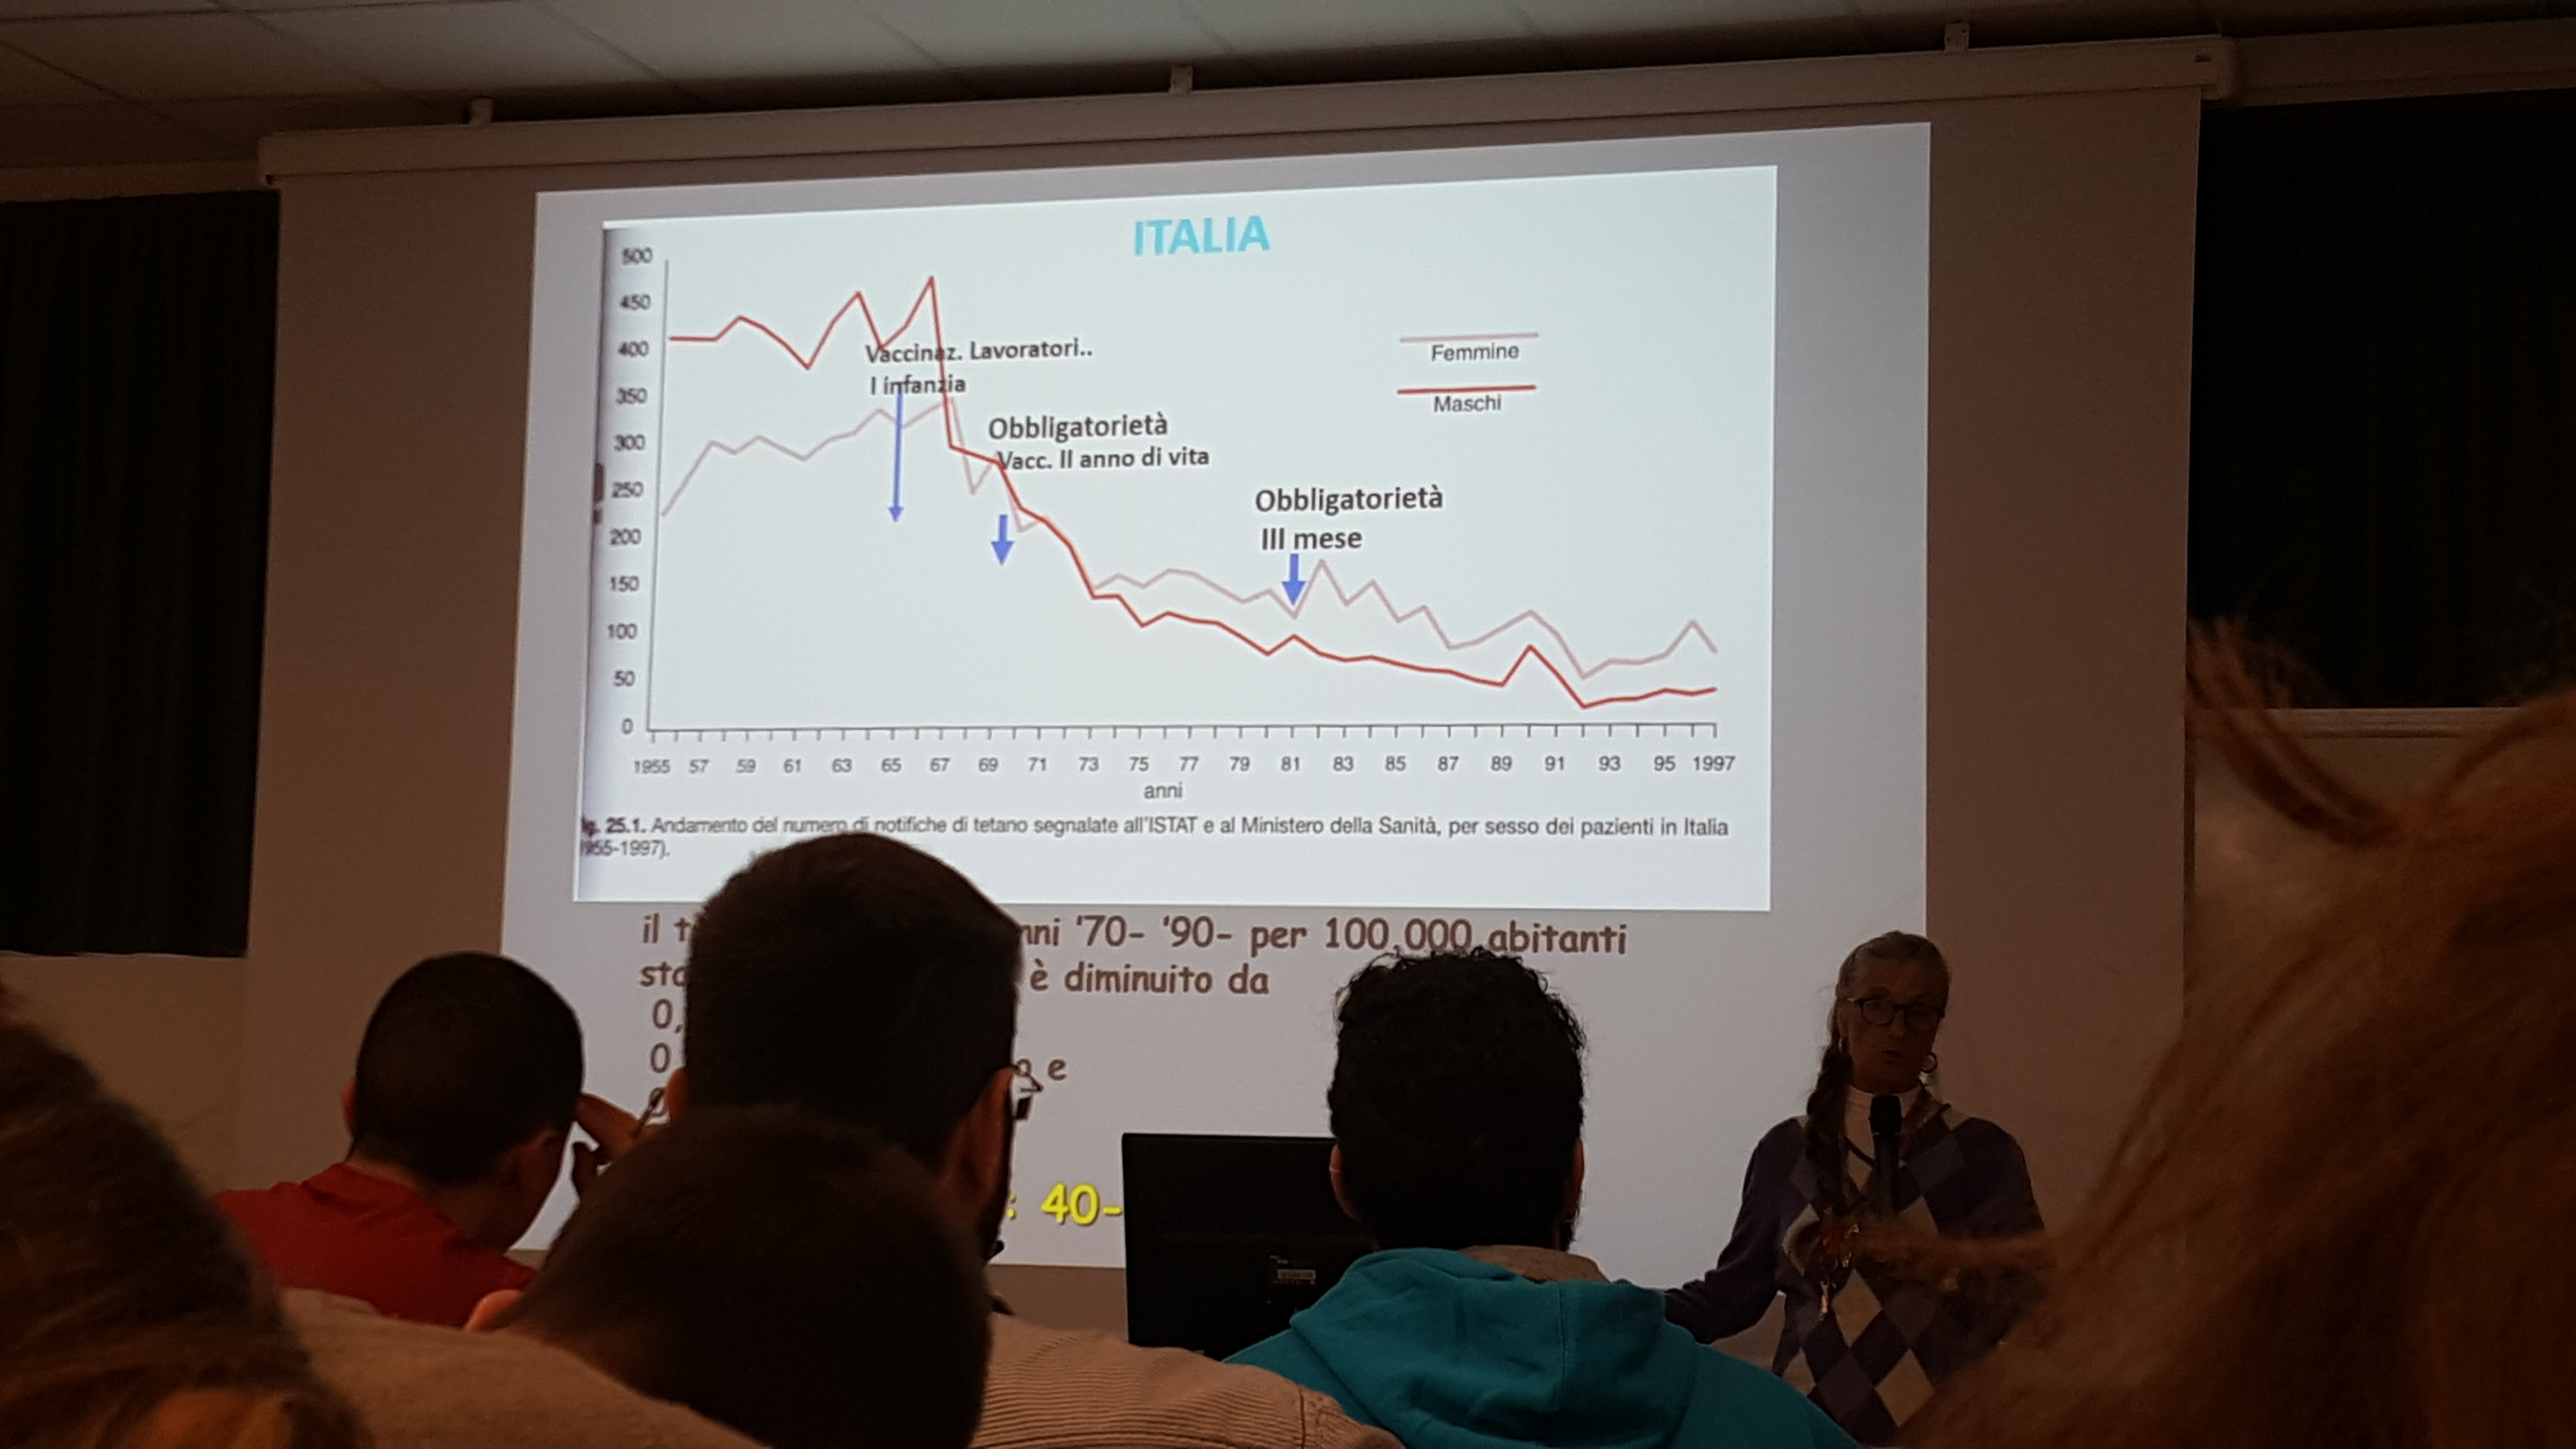
\includegraphics[width=0.7\textwidth]{06/image6.jpeg}
\end{figure}

  Come si spiega questa inversione di tendenza? La vaccinazione del
  maschio è sempre stata più consolidata rispetto a quella delle donne
  sia per la leva militare obbligatoria prima e poi per via delle
  attività lavorative mentre per le donne non sono mai esistiti degli
  step di rivaccinazione per cui sono più esposte al rischio.

  Oggi quindi in Italia il tetano è maggiormente diffuso nelle donne
  però nella popolazione anziana:

\begin{itemize}
\item
  Il fattore età si spiega con la riduzione dell'immunità acquisita con
  le vaccinazioni nell'infanzia. Si tratta di un qualcosa di inevitabile
  soprattutto se non vengono effettuati i richiami ogni 10 anni
\item
  La maggior prevalenza nel sesso femminile invece dipende come già
  detto dal fatto che si immunizzano meno dei maschi e hanno maggiore
  probabilità di svolgere attività all'aria aperta che sono
  potenzialmente pericolose (attività di giardinaggio, ma anche pulendo
  certe verdure contenenti spine).
\end{itemize}
  Oggi si registrano circa 60 casi su 60 milioni di abitanti: sono pochi
  però è un problema perché abbiamo a disposizione una vaccinazione
  efficace che potrebbe benissimo evitare queste morti.

  Le tipologie di tetano in base al tipo d infezione sono: tetano
  traumatico, tetano medico, tetano chirurgico, tetano neonatale, tetano
  puerperale e tetano post-aborto

   \begin{figure}[!ht]
\centering
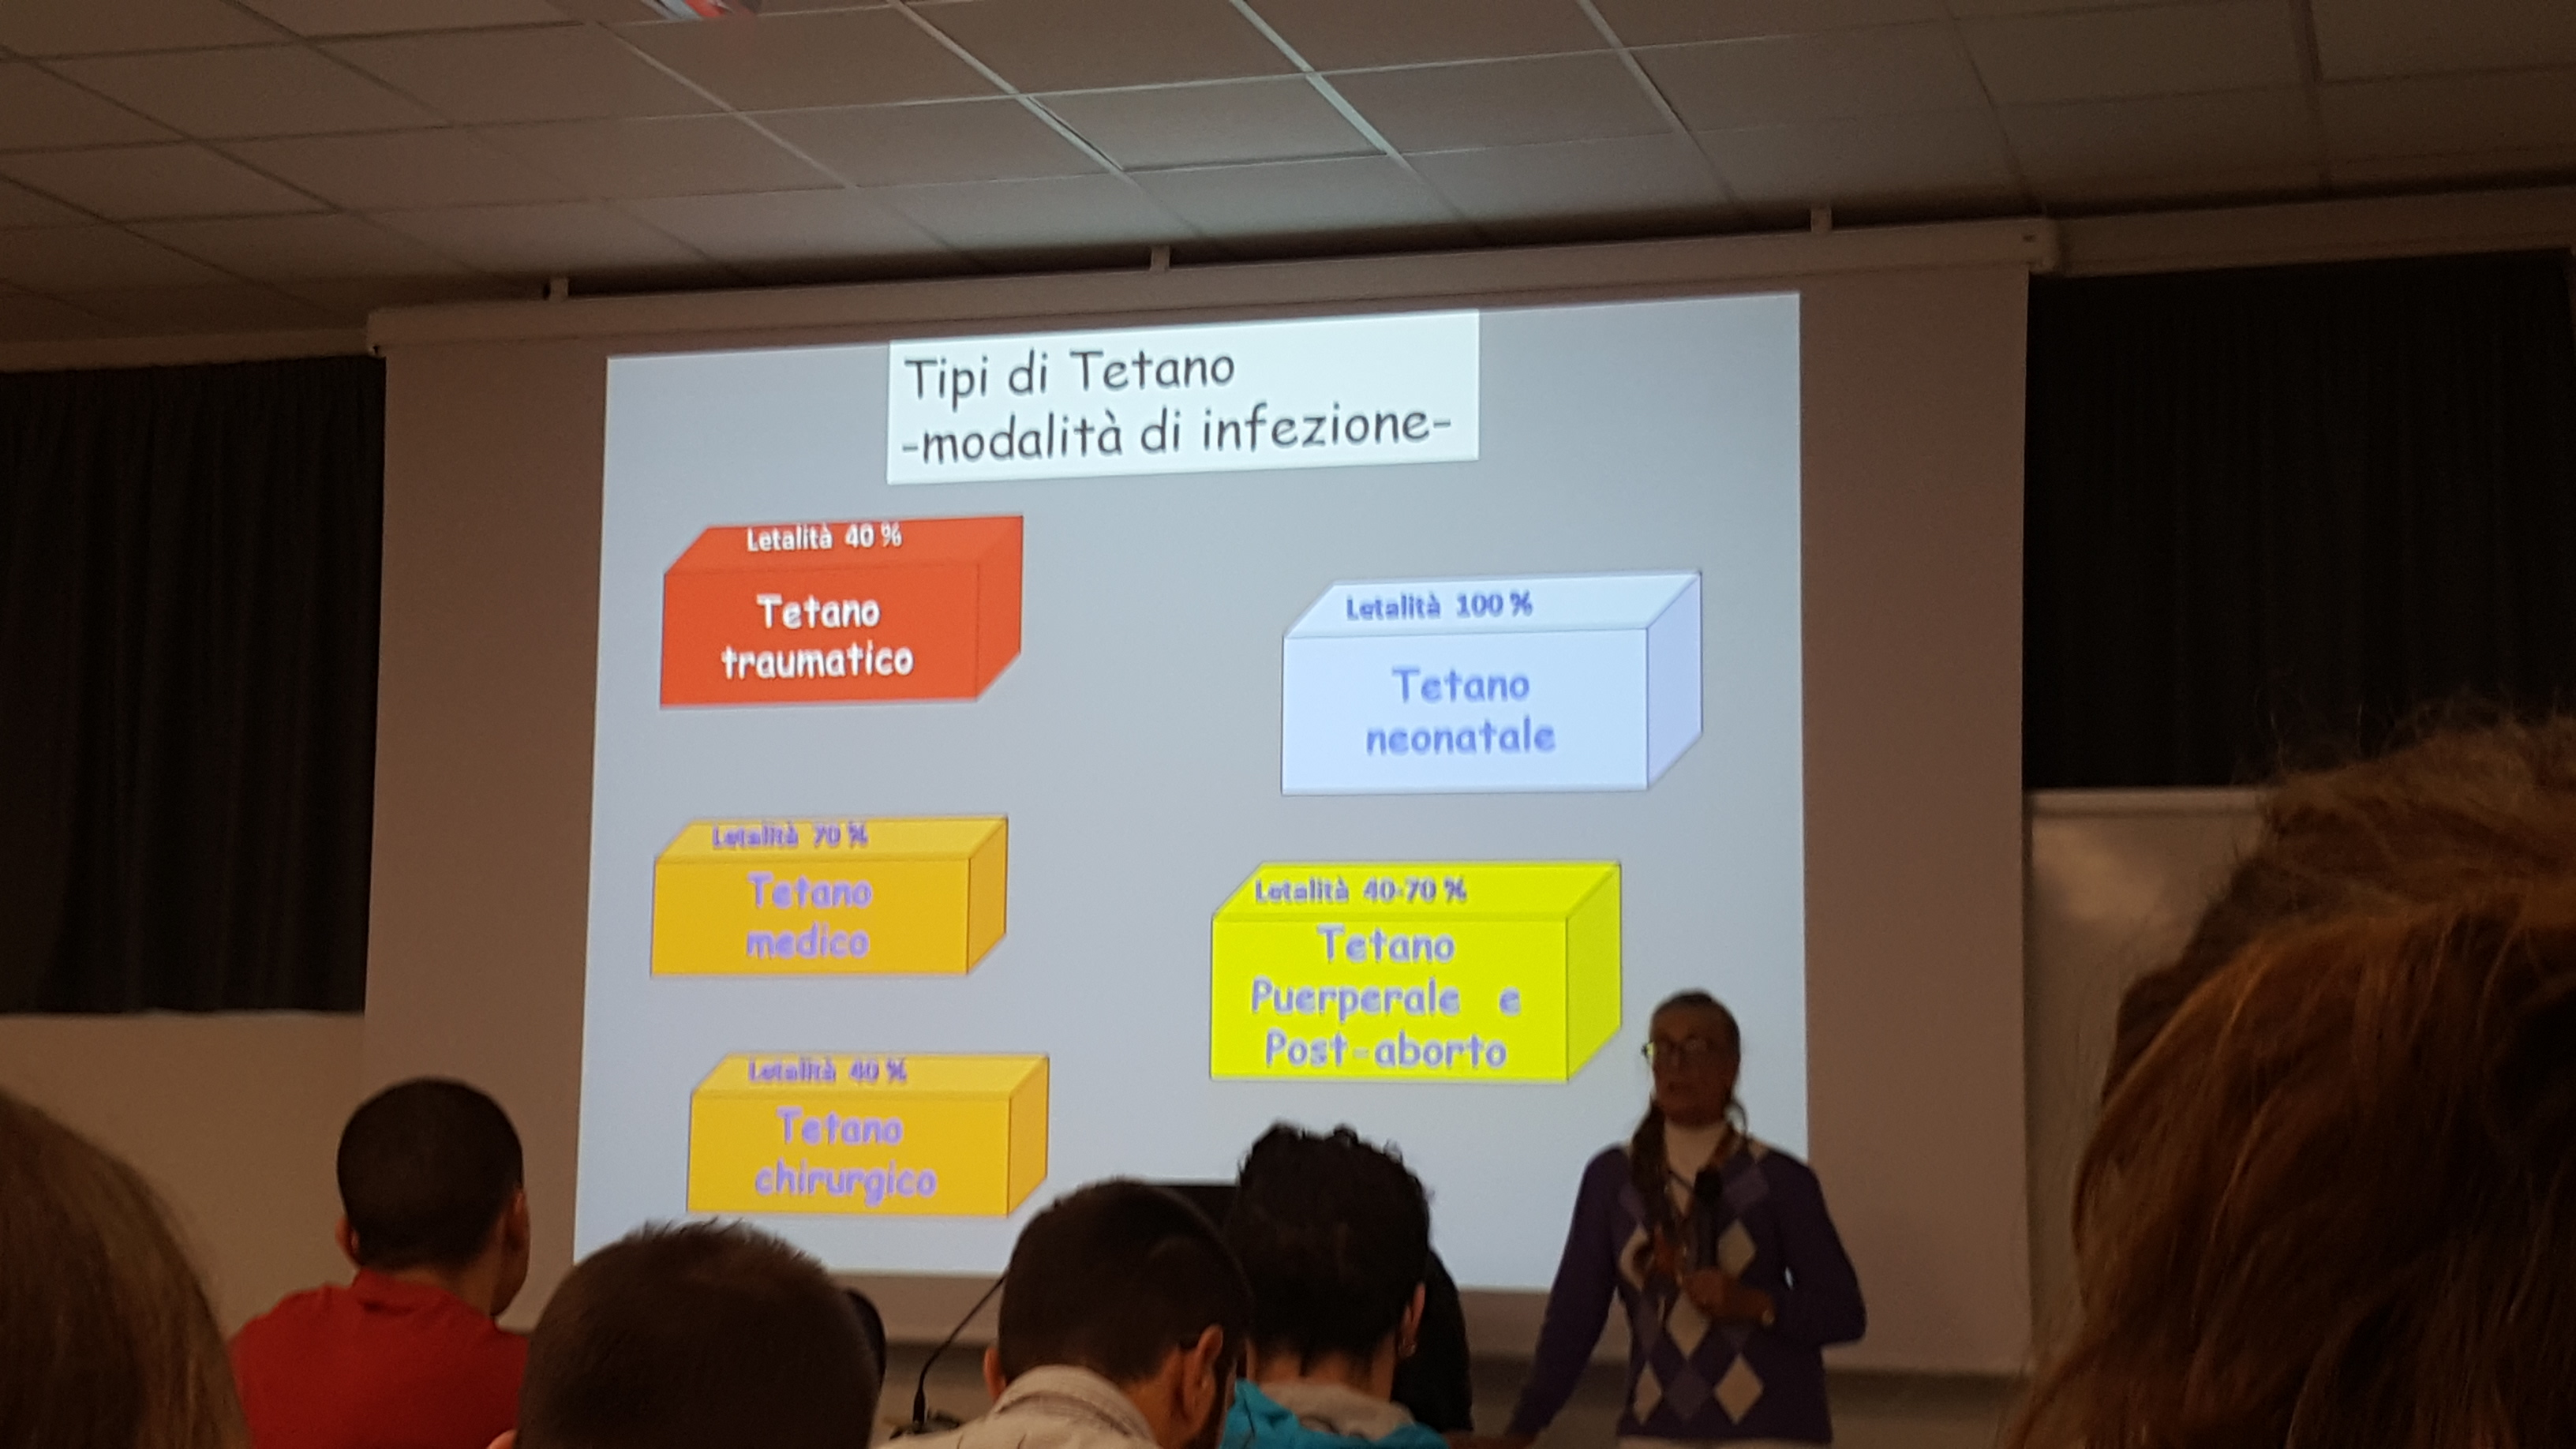
\includegraphics[width=0.7\textwidth]{06/image7.jpeg}
\end{figure}

  Da noi è prevalente se non esclusiva la forma traumatica mentre in
  altre realtà come i paese in via di sviluppo sono ancora importanti le
  forme neonatali, puerperali e post-aborto. Qualunque trauma, ferita,
  puntura è potenzialmente a rischio di infezione tetanica.

  Dal 1995 quando i casi di tetano neonatale erano ancora presenti in 52
  paesi, c'è stata un progressiva riduzione e a oggi sono 24 i paesi in
  cui questa forma di tetano neonatale è ancora presente ed è legata ad
  una cattiva pratica ostetrica che causa generalmente contaminazione
  ambientale del cordone ombelicale e che da una forma con letalità del
  100\%.

\subsubsection{Modalità di contagio e clinica}

  E' un batterio sporigeno e anaerobio e queste due caratteristiche lo
  rendono assolutamente pericoloso per noi.

\begin{itemize}
\item
  Sporigeno significa che sopravvive nell'ambiente e in questo caso
  potremmo dire all'infinito perché i tempi di sopravvivenza della spora
  sono veramente lunghi e sopravvive nel suolo, polvere, scarti e sulle
  superfici arrugginite
\item
  E' un batterio che teme l'ossigeno infatti è anaerobio e sopravvive
  nell'ambiente esterno solo grazie alla produzione di spore
\end{itemize}
  E' tipicamente un batterio non invasivo, si localizza nel punto di
  penetrazione e lì se trova le condizioni di anaerobiosi germina e dà
  luogo alla tossina che è la tetanospasmina che è una tossina
  potentissima e responsabile della sintomatologia neurologica. La dose
  letale stimata per Kg è 2,5 ng: una quota talmente bassa da non
  rappresentare uno stimolo adeguato per il sistema immunitario perciò a
  seguito dell'infezione non abbiamo l'immunità che invece stimoliamo
  con una dose adeguata che è quella presente nel vaccino. Ha uno
  spiccato tropismo per il sistema nervoso e in particolare per le corna
  anteriori del midollo spinale, si fissa in modo irreversibile e non
  può essere neutralizzato da anticorpi in questa fase. La tossina
  blocca la conduzione dell'impulso nervoso inibitorio e in particolare
  blocca il rilascio di Ach così che ad ogni contrazione si contraggano
  anche i muscoli antagonisti e si ha una contrattura spastica che può
  anche portare a morte a seconda della muscolatura coinvolta. Penetra
  prevalentemente attraverso lesioni cutanee e se nell'ambiento in cui
  penetra c'è una ridotta tensione parziale di ossigeno germina. La
  tossina va in circolo per via neuronale e linfo-ematica. Il periodo di
  incubazione è molto lungo: da qualche giorno a 1 mese. Ci sono varie
  forme di tetano, ma la più importante è la generalizzata con sintomi
  che si propagano in direzione ascendente: spasmi e rigidità muscolare
  che porta a morte nel 40-60\% dei casi quindi 4-6 casi su 10 vanno
  incontro a morte.

\subsubsection{Prevenzione e profilassi}

  È una malattia soggetta a notifica obbligatoria. Non richiede
  particolari accertamenti diagnostici perché è piuttosto caratteristica
  nella forma in cui si presenta. Tali accertamenti sono condotti solo
  in caso ci siano problemi medico-legali o per necessità di studio
  epidemiologico. Importante la disinfezione intesa come quella della
  ferita perché non c'è rischio di trasmissione inter-umana. Quindi
  toilette della ferita e immunoprofilassi attiva e passiva ovvero
  immunoglobuline specifiche per la tossina tetanica.

  Il vaccino è disponibile dagli anni 20-30. È sempre costituito da
  un'anatossina potenziata con un adiuvante che stimoli il sistema
  immunitario. Ci sono tanti vaccini che hanno la componente tetanica
  proprio per la sua persistenza come problema nella società. Per i
  bambini abbiamo:

\begin{itemize}
\item
  Il vecchio bivalente
\item
  Trivalente: difterite, tetano e pertosse
\item
  Più recenti invece sono il penta e esavalente gli stessi vantaggi dei
  singoli vaccini in termini di immunità e in più il vantaggio di una
  singola somministrazione
\end{itemize}
  Per gli adulti invece abbiamo:

\begin{itemize}
\item
  Il monovalente che vorremmo non esistesse più perché è meglio
  promuovere altre soluzioni.
\item
  Il bivalente: tetano + dose ridotte per la difterite
\item
  Trivalente: tetano + dose ridotta per difterite + pertosse
\item
  Tetravalente: tetano + difterite + pertosse + poliomielite per
  situazioni particolari
\end{itemize}
  La vaccinazione è stata introdotta negli anni 20-30 e all'inizio solo
  per i militari poi dagli anni 60 è stata estesa anche ai bambini nel
  secondo anno di vita e ai lavoratori agricoli. Dal 1968 è stata
  anticipata al primo anno di vita associata a quella per la difterite e
  la pertosse. Inoltre la vaccinazione è:

\begin{itemize}
\item
  Obbligatoria per tutti gli iscritti al CONI
\item
  Obbligatoria per alcune categorie professionali: allevatori di
  bestiame, asfaltatori, cantonieri, conciatori, fantini, fornaciai,
  lavoratori agricoli, lavoratori del legno, metalmeccanici e lavoratori
  edili
\item
  Fortemente consigliata per tutti gli adulti perché se manteniamo
  sufficientemente elevato il titolo anticorpale, riduciamo il rischio
  di contrarre l'infezione
\end{itemize}
  La scheda dell'infanzia prevede 4 somministrazioni e l'ultima intorno
  ai 12 anni perché la protezione minima del vaccino è di 10 anni: in
  realtà non è così perché in alcuni dura molto di più però in altri
  anche di meno perciò si è scelto il limite temporale inferiore.
  Facendo una vaccinazione tra i 12-13 anni ho una protezione fino ai
  22-23 anni e da lì in poi entra in gioco la coscienza individuale o
  l'obbligatorietà per certe categorie professionali.

  Per l'adulto sono previste di base tre dosi di cui la prima al tempo
  0, la seconda dopo 3 mesi e la terza dopo 6 e anche qui è previsto un
  richiamo ogni 10 anni.

  Gli effetti collaterali sono sovrapponibili a quelli della difterite
  però un po' meno perché è meno reattogeno il preparato.

  L'Immunoprofilassi è sempre un intervento di emergenza, ha effetto
  protettivo nell'immediato però non è duraturo come effetto.

  \begin{figure}[!ht]
\centering
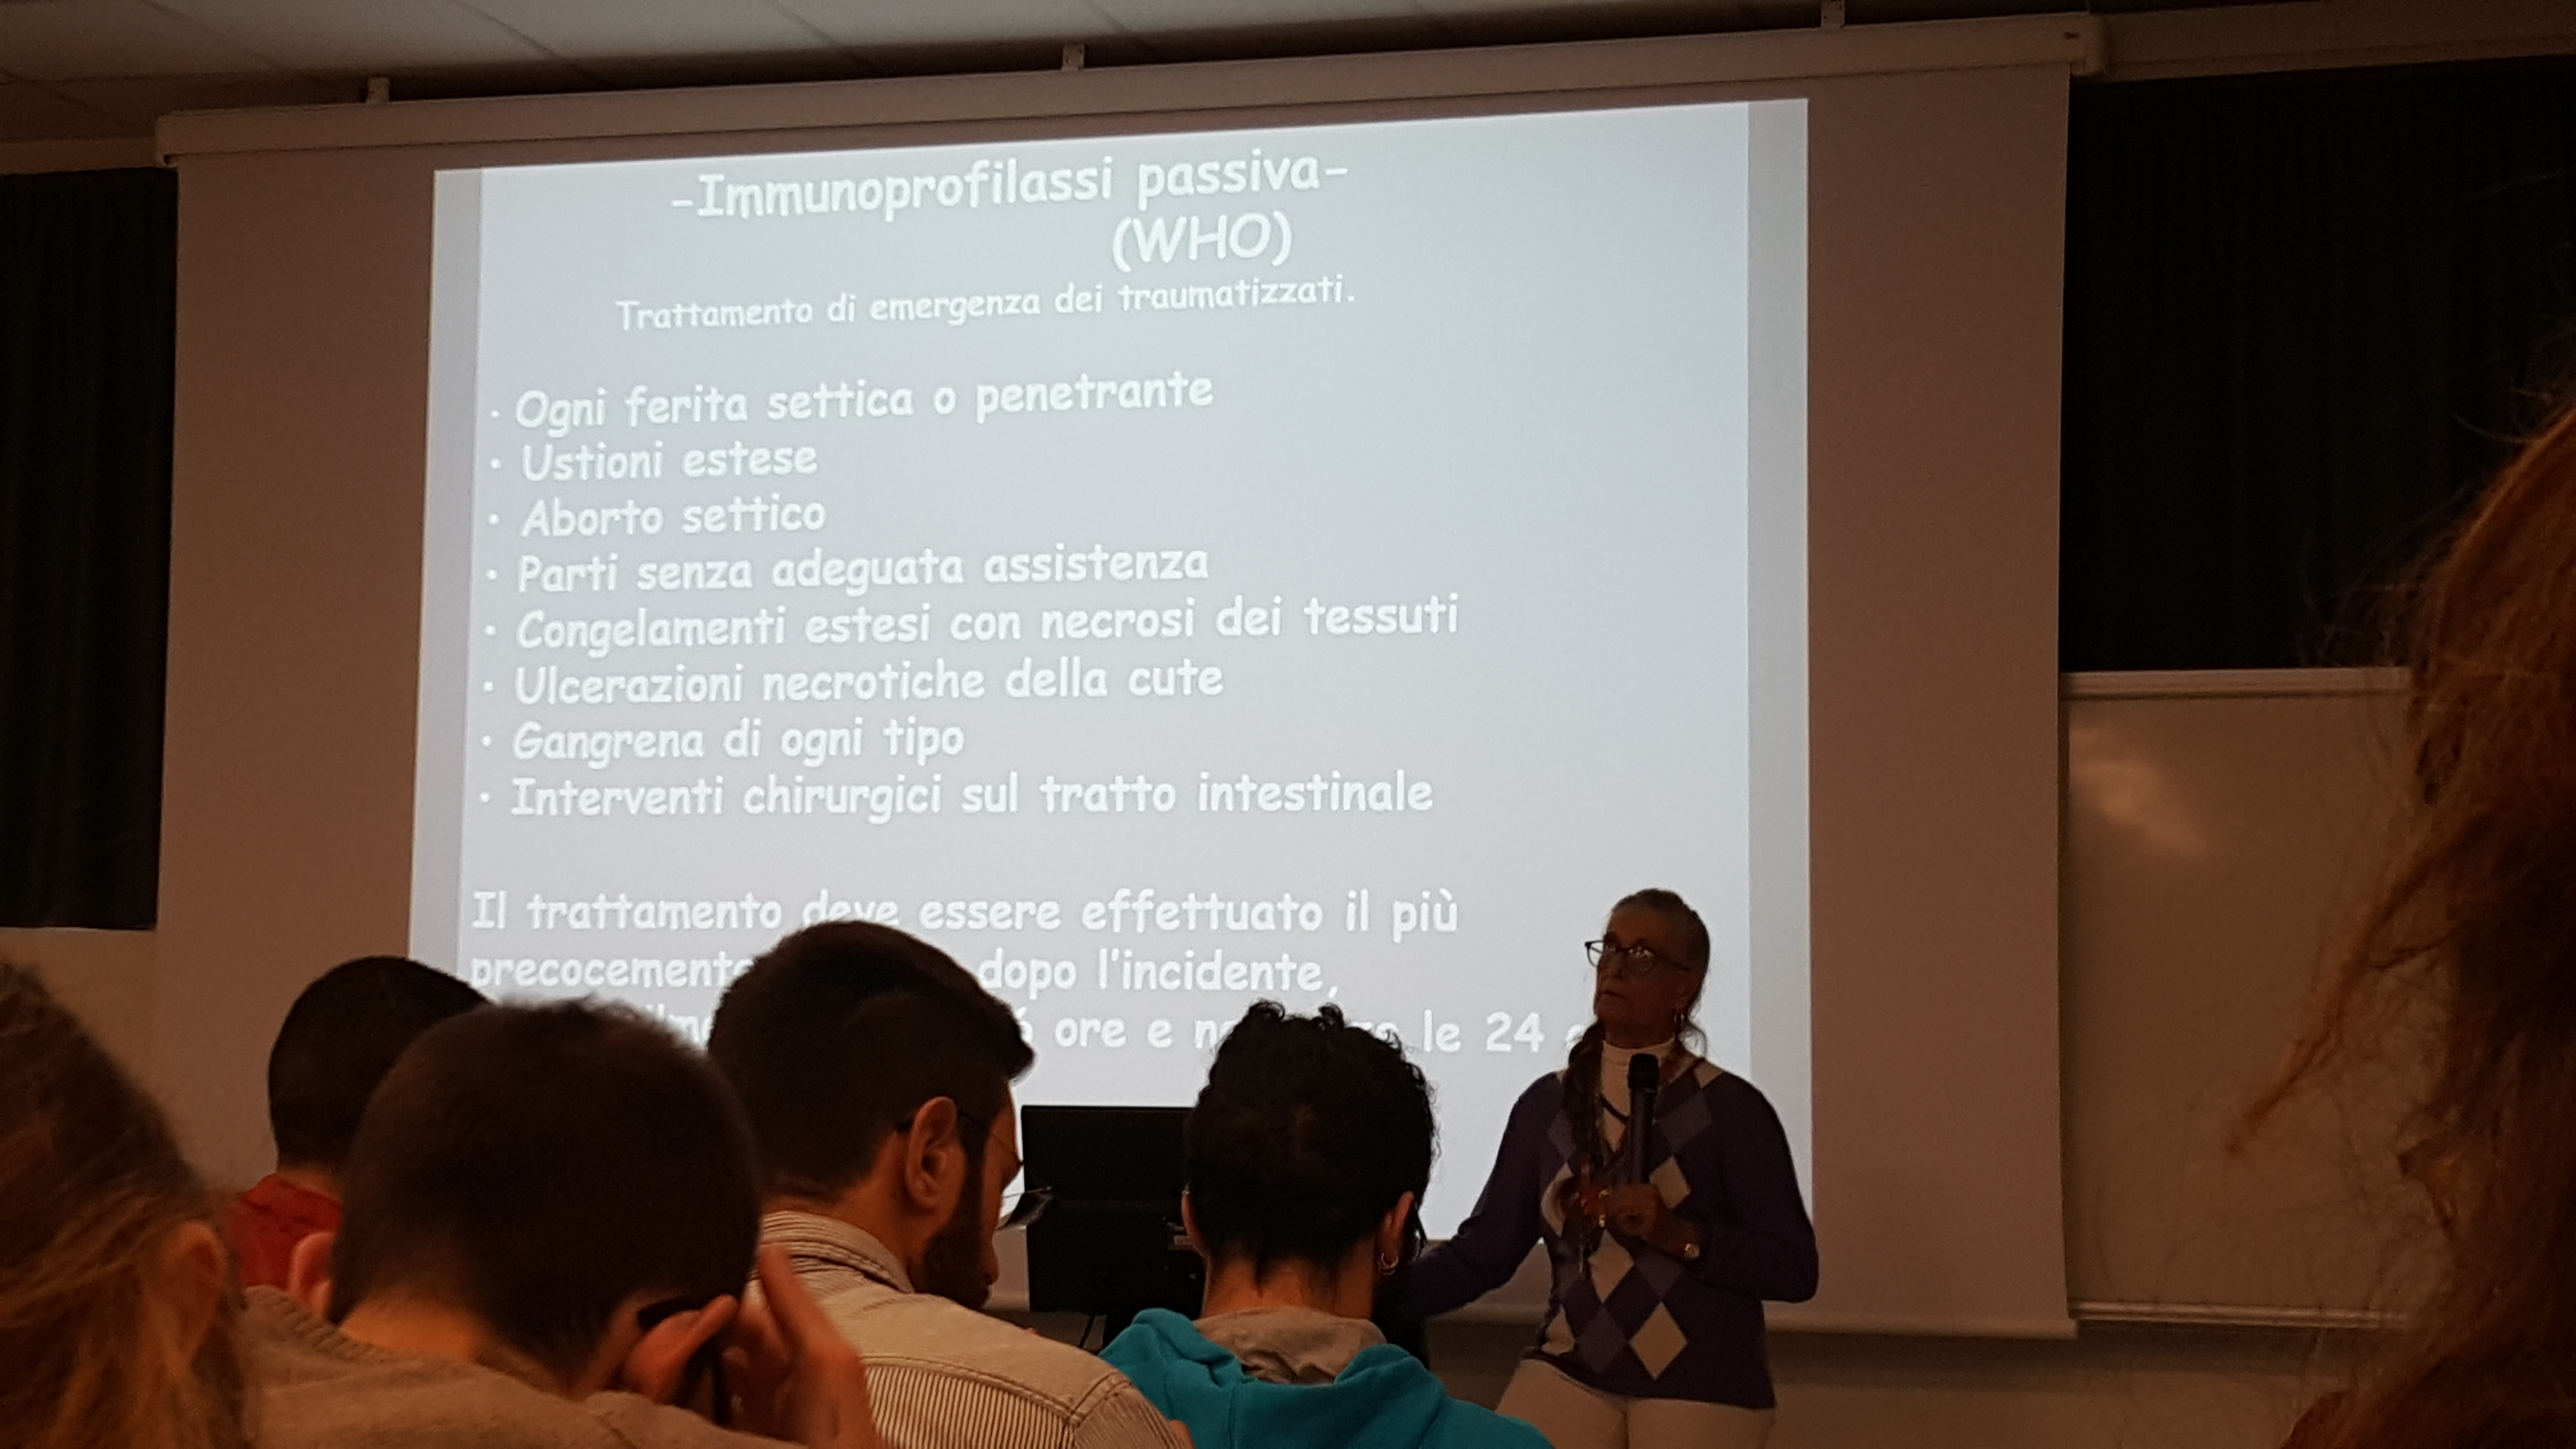
\includegraphics[width=0.7\textwidth]{06/image8.jpeg}
\end{figure}

  Non confondiamo l'immunizzazione passiva con la vaccinazione: non sono
  la stessa cosa! Con l'immunizzazione passiva il soggetto è protetto
  nell'immediato, ma poi ritorna nella stessa condizione di
  suscettibilità precedente la somministrazione di IgG. Si tratta di IgG
  ad alto titolo quindi preparati altamente specifici per il tetano. Vi
  sono delle condizioni legate soprattutto al tipo di lesione che
  delineano una condizione di necessità per quanto riguarda la
  somministrazione delle immunoglobuline. Tanto più è precoce la
  somministrazione più le IgG sono efficace: ideale entro le sei massimo
  entro le 24 ore. Su qualunque ferita deve essere eseguita una toilette
  ben fatta: lavaggio e rimozione di detriti, schegge, tessuti quindi
  pulizia e eventualmente rimozione di tessuto necrotico. A questo punto
  si procede con la disinfezione e l'acqua ossigenata è ottima perché
  ruba ossigeno e protegge anche da altre infezioni. Dopodiché
  immunoglobuline e/o vaccino. Le indicazioni per l'adulto devono tenere
  conto dello stato vaccinale quindi immunitario e della tipologia di
  ferite (lieve quindi a basso rischio o significativa quindi ad alto
  rischio). Prendiamo come riferimento lo stato vaccinale perché non
  abbiamo tempo di andare a valutare il titolo anticorpale quindi è più
  pratico e più veloce andare a controllare la scheda vaccinale

\begin{itemize}
\item
  Se non c'è modo di controllare la scheda vaccinale o non c'è certezza,
  quel soggetto viene considerato a rischio e a prescindere dalla ferita
  si procede con la vaccinazione (tre dosi: prima, dopo 3 mesi e dopo 6)
\item
  Se è lieve basta la vaccinazione
\item
  Se è grave anche le immunoglobuline
\item
  Se l'ultima somministrazione vaccinale risale a più di dieci anni fa
  allora si somministra il vaccino e le immunoglobuline
\item
  Se l'ultima somministrazione vaccinale risale a un periodo compresa
  tra 5 e 10 anni fa allora viene somministrata la dose di richiamo e le
  immunoglobuline
\item
  Se l'ultima somministrazione risale a meno di 5 anni fa viene
  somministrata una sola dose solo se c'è elevato rischio di infezione
  altrimenti non si somministra nulla.
\end{itemize}

\subsection{Pertosse}

  La pertosse è una malattia altamente contagiosa il cui agente
  eziologico è la Bordetella Pertussis. E' nota da sempre ed è stata
  introdotta ormai da molti anni la vaccinazione, ma nonostante questo
  abbiamo ancora 40 milioni di casi l'anno al mondo e di questi circa
  350 mila muoiono. E' quindi una malattia a diffusione mondiale con
  andamento epidemico. Il passo tradizionale prima della vaccinazione
  erano le epidemie ogni 3/5 anni a inizio primavera e inverno. È ancora
  una malattia molto presente e pericolosa seppure in determinate fasce
  d'età. Un altro dato importante è quello riguardante l'immunità:

\begin{itemize}
\item
  Quella naturale che comincia a ridursi dai 4 anni e poi questa
  riduzione è progressiva fino ai 20 anni quando sostanzialmente si
  perde
\item
  Quella artificiale cioè indotta dal vaccino è duratura, ma meno di
  quella naturale infatti comincia a decadere a partire dai 4 anni e
  mediamente si annulla intorno ai 12 anni
\end{itemize}
  E' bene ricordarlo per meglio comprendere le basi delle strategie
  vaccinali odierne.

  E' un bacillo molto labile nell'ambiente e viene rapidamente
  inattivato da particolari condizioni ambientali e climatiche (troppo
  caldo, troppo freddo, ecc.). E' la classica malattia infettiva
  altamente contagiosa e a trasmissione interumana.

  Sono necessari alcuni cenni sulla struttura del patogeno che servono
  per comprendere meglio la logica dei vaccini. Gli antigeni importanti
  per la patogenesi del danno e che dobbiamo/possiamo utilizzare per
  l'immunizzazione passiva sono:

\begin{itemize}
\item
  La tossina pertussica che è un fattore promuovente la linfocitosi. E'
  un esotossina termolabile con molte attività biologiche e certamente è
  il perno del danno biologico
\item
  Pertactina che è sempre presente in tutti i ceppi virulenti e
  favorisce l'adesione alle cellule bersaglio che sono le cellule
  epiteliali (favorisce però non è determinante)
\item
  Agglutinasi varie
\item
  Emoagglutinina filamentosa che ha un componente di parete che è la
  chiave per l'aggancio della Bordetella alle cellule dell'apparato
  cigliato delle vie aeree
\end{itemize}
  La tossina pertussica, la pertactina e l'emoagglutinina filamentosa
  sono antigeni perché immunogeni e aiutano nella difesa/protezione
  dall'infezione.

  E' classicamente un infezione dell'età pediatrica. Il patogeno penetra
  per via aerea, aderisce alle cellule dell'epitelio respiratorio
  bronchiale dove si localizza. In questa sede provoca flogosi catarrale
  dell'epitelio e necrosi a livello della zona basale probabilmente per
  azione della tossina. Ne deriva irritazione della mucosa, accesso
  parossistico e dopo di ciò c'è la diffusione della tossina con le
  conseguenti manifestazioni sistemiche.

\subsubsection{Clinica}
  Ha un periodo di incubazione discreto ovvero 7-10 giorni mediamente.
  Di base è una flogosi delle alte vie respiratorie che si presenta con:

\begin{itemize}
\item
  Tosse aspecifica e stizzosa
\item
  Spasmi parossistici con accessi non intervallati da atti respiratori e
  conseguente sibilo caratteristico
\item
  Spesso vomito dopo la tosse
\item
  Febbre modica (mediamente)
\end{itemize}
  Ha un lungo decorso e prevede diverse fasi:

\begin{itemize}
\item
  Stadio catarrale (1-2 settimane)
\item
  Stadio ascessuale (1-6 settimane)
\item
  Convalescenza (settimane o mesi)
\end{itemize}
  Sono possibili le così dette forme fruste (asintomatiche o
  pauci-sintomatiche) che sono molto importanti perché:

\begin{itemize}
\item
  Non sono evidenti, ma creano problemi perché sono soggetti contagiosi
\item
  Sono forme dell'adulto che possono così infettare i bambini
\end{itemize}
  La letalità della malattia è infatti elevata nel lattante a causa di
  complicanze:

\begin{itemize}
\item
  Respiratorie: crisi d'apnea nel 50\% dei casi e broncopolmoniti nel
  20\% dei casi
\item
  Neurologiche nei bambini entro il primo anno di vita come conseguenza
  dei parossismi e sono molto gravi soprattutto se le apnee sono
  prolungate. Si tratta per lo più di convulsioni nel 1 \% dei casi e
  encefalopatia nello 0.3\%
\item
  Decessi nell'1\% dei casi
\end{itemize}
  La gravità è stimata inversamente proporzionale all'età quindi sarà
  particolarmente severa nei lattanti e nella maggior parte dei casi
  richiede l'ospedalizzazione. Dobbiamo temere la pertosse per il
  lattante.

\subsubsection{Modalità di trasmissione e contagio}

  Sorgente d'infezione è l'uomo come:

\begin{itemize}
\item
  Malato palese
\item
  Portatore sano o asintomatico (forme fruste) che è un forte diffusore
\item
  Portatore precoce che è un eliminatore importante
\end{itemize}

  E' un problema di tutti i paese industrializzati quello dell'infezione
  dell'adulto ed è problematico per i bambini. I dati riportano 25 mila
  casi con due picchi: bambini al di sotto dell'anno di vita e bambini
  di 12-14 anni. Queste sono le fasce d'età più importanti. Continua
  quindi a serpeggiare con casi isolati di pertosse e piccoli focolai e
  se li rapportiamo allo stato vaccinale, sono bambini non vaccinati o
  vaccinati in ritardo perché anche la sequenza delle vaccinazioni è
  importante nella prevenzione del danno quindi a volte le vaccinazioni
  non seguono l'iter corretto oltre a non essere effettuate. La
  contagiosità è molto elevata e molto persistente nel tempo però se un
  bambino è trattato con eritromicina si abbatte la contagiosità.
  Nell'adulto la malattia è lieve o non presente clinicamente. Abbiamo a
  disposizione pochi dati in riferimento a gli adulti proprio perché si
  presenta in forma lieve. I pochi dati a disposizione ci dicono che
  circa il 7\% degli adulti è andato incontro a infezione e non è un
  dato da poco se si considera che gli adulti sono la fonte di infezione
  più importante per i bambini. La contagiosità è molto importante in
  termini di durata: dal periodo catarrale fino a 3 settimane dopo la
  comparsa dei sintomi quindi c'è un lungo periodo di eliminazione del
  patogeno nel malato e presumiamo avvenga anche nel sano però
  ovviamente non abbiamo gli step di malattia visti. Il malato lo
  possiamo però controllare anche se sono molto alti i costi di
  gestione.

\subsubsection{Prevenzione e profilassi}

  E' prevista la denuncia, ma non l'isolamento nel senso che non è
  previsto per legge però è bene tenere il bambino malato lontano da
  altri bambini soprattutto lattanti. Se viene riconosciuto come
  malattia conclamata sappiamo sarà infettante per i prossimi 7 giorni
  dopo trattamento farmacologico quindi è bene limitare i contatti in
  questa fase. L'inchiesta epidemiologica serve per attuare la
  chemioprofilassi per contatti e conviventi. La disinfezione è una
  pratica comune, ma dal momento che il batterio è molto fragile una
  blanda disinfezione è già sufficiente.

  Per quanto riguarda il vaccino si tratta di un vaccino inattivato
  quindi Bordetella uccise con una massa molto elevata nel preparato.
  Con i preparati inizialmente adoperati si registrarono rari casi di
  encefalopatia per cui c'è stata una riduzione della pratica vaccinale
  con il ritorno di epidemie. Questo però ha anche intensificato la
  ricerca e oggi abbiamo a disposizione due preparati (degli anni 80):
  uno europeo e uno giapponese. Sono entrambi vaccini contenenti
  componenti antigeniche in grado di conferire immunità quindi si tratta
  di un vaccino purificato, a componenti e molto efficace con effetti
  collaterali molto modesti. L'europeo è dei ricercatori italiani e la
  differenza è che l'inattivazione della tossina pertussica è ottenuta
  mediante tecniche di ingegneria genetica e non chimicamente con il
  formolo come nella variante giapponese. Tutti i vaccini contengono
  sempre almeno due componenti: la tossina pertussica e almeno uno degli
  altri due antigeni. I vaccini che usiamo per i bambini sono:

\begin{itemize}
\item
  Il trivalente
\item
  Il penta-esavalente per bambini
\end{itemize}
  Per gli adulti invece si usa il trivalente.

  La scheda vaccinale è la solita: 3 somministrazioni di cui la prima
  nel secondo mese del primo anno di vita e richiami al sesto e
  dodicesimo mese. Gli effetti collaterali sono piuttosto blandi e
  locali. Oggi l'obiettivo è la vaccinazione dei nuovi nati e poi dei
  giovani adulti e adulti per mantenere elevati standard di protezione,
  ridurre la circolazione del batterio e ridurre la probabilità per i
  soggetti a rischio (neonati) di essere infettati. Nell'adulto quindi
  non sarebbe importante vaccinare per la pertosse, ma lo si fa per
  proteggere i soggetti a rischio e sarebbe ideale vaccinare genitori,
  parenti, medici, adolescenti a contatto con bambini e neonati.